\chapter{Stokes formalization blueprint}

This blueprint is a dependency map for the Lean 4 Stokes project.  The unit of
work is a public definition, lemma, theorem, or a deliberately named future
interface.  Green nodes in the figures are already implemented in Lean; orange
nodes are fieldized blockers whose constructors exist but whose geometric or
measure-theoretic instances are still genuine work; blue nodes are open theorem
targets intended to be small enough for independent assignment.

The current formalized stack already reaches boundary-chart local Stokes.  The
remaining work is not "prove Stokes" as one block: it is the finite-cover,
partition-of-unity, and global-integral assembly layer recorded in
\Cref{sec:global_assembly}.

\clearpage
\begin{landscape}
\begin{figure}[p]
  \centering
  \noindent\makebox[\linewidth][c]{%
    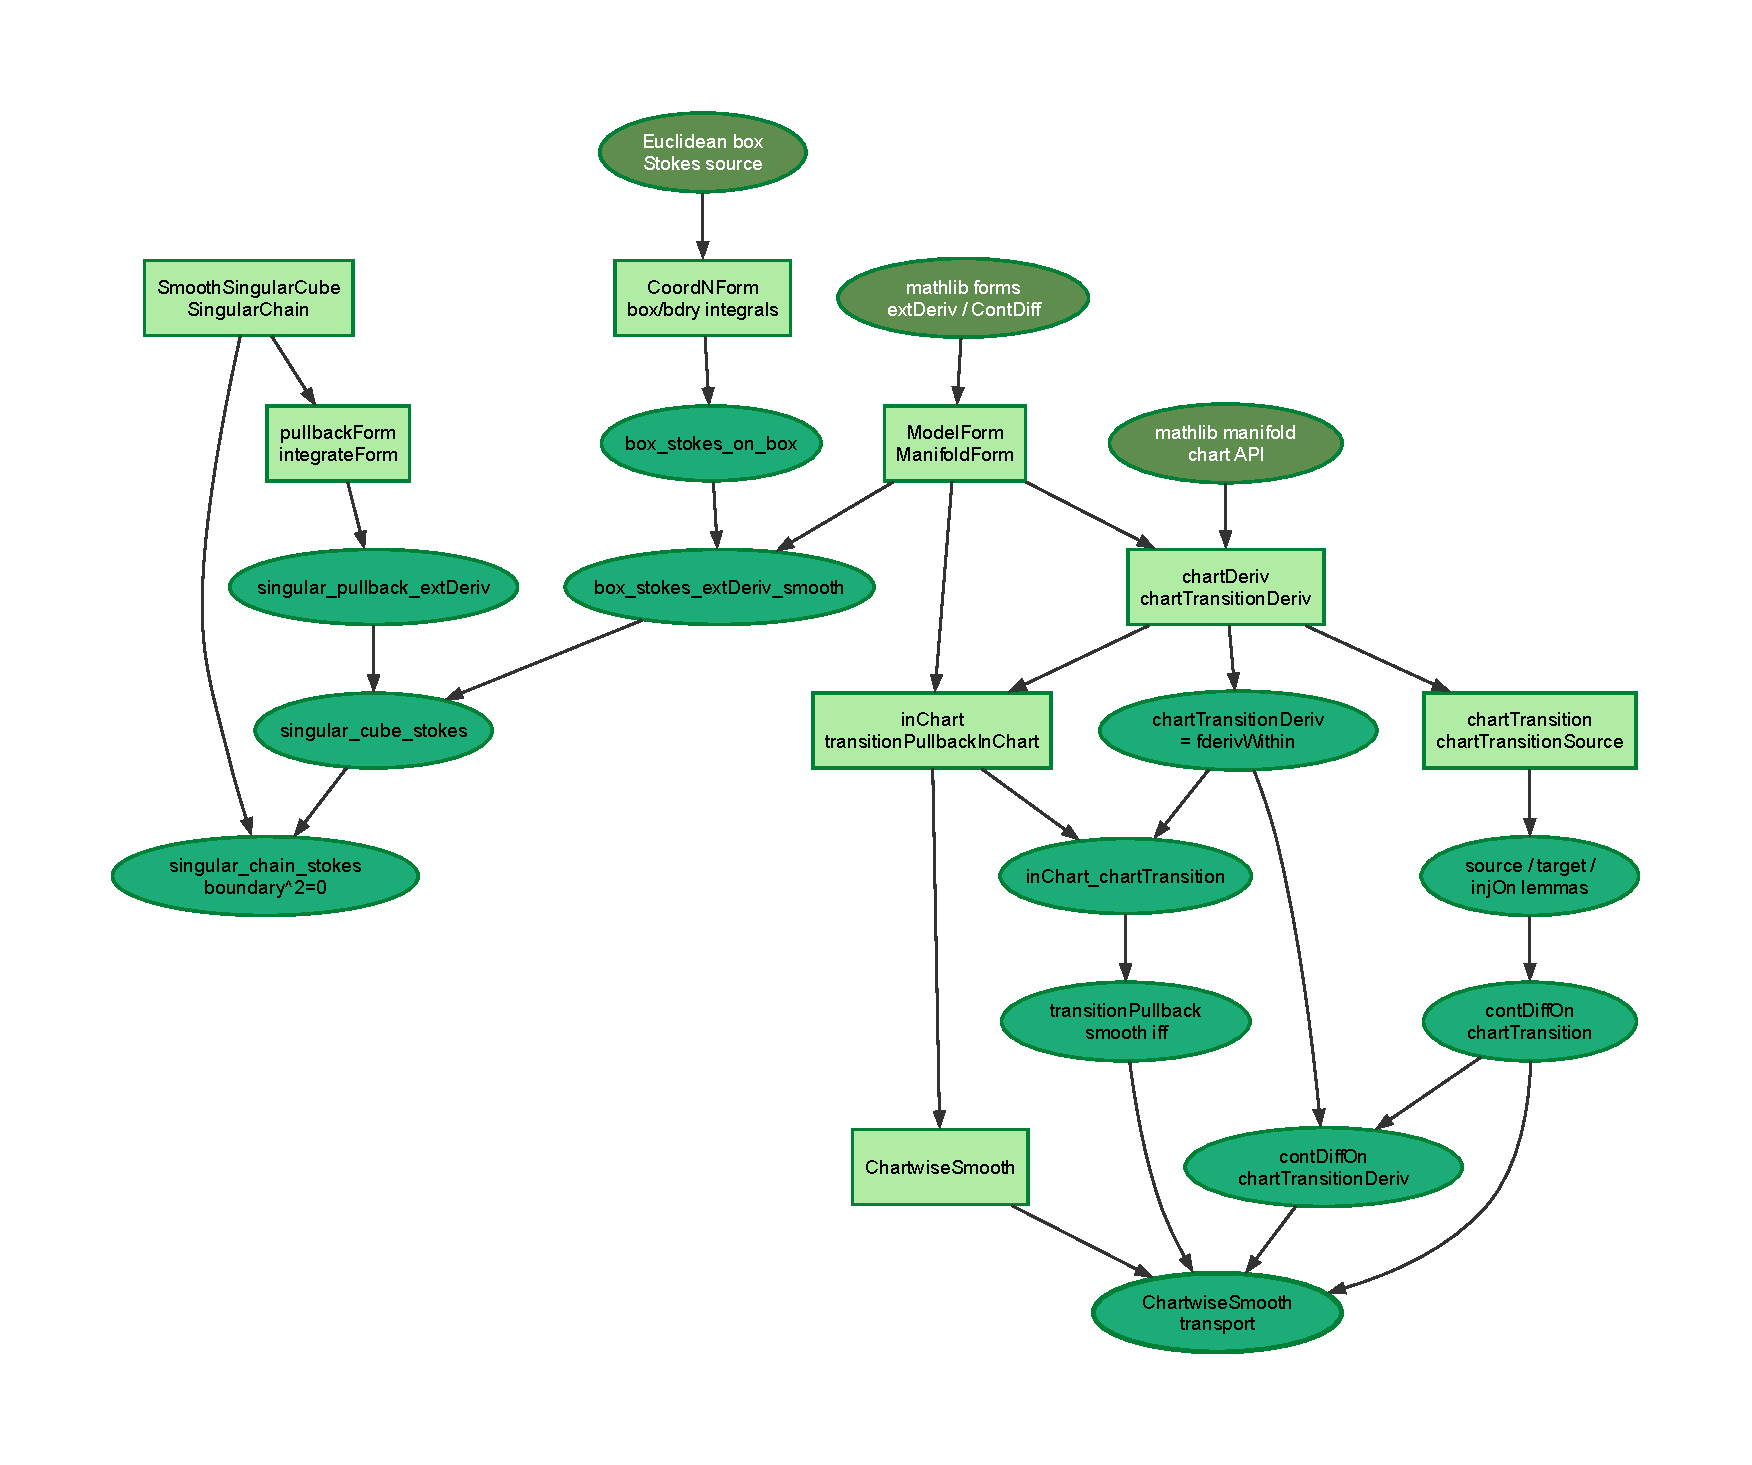
\includegraphics[width=0.90\paperheight,height=0.62\paperwidth,keepaspectratio]
      {figures/stokes-core-graph.pdf}}
  \caption{Core Euclidean, singular-cube, and chart-representative API.}
  \label{fig:stokes_core_graph}
\end{figure}
\end{landscape}

\begin{landscape}
\begin{figure}[p]
  \centering
  \noindent\makebox[\linewidth][c]{%
    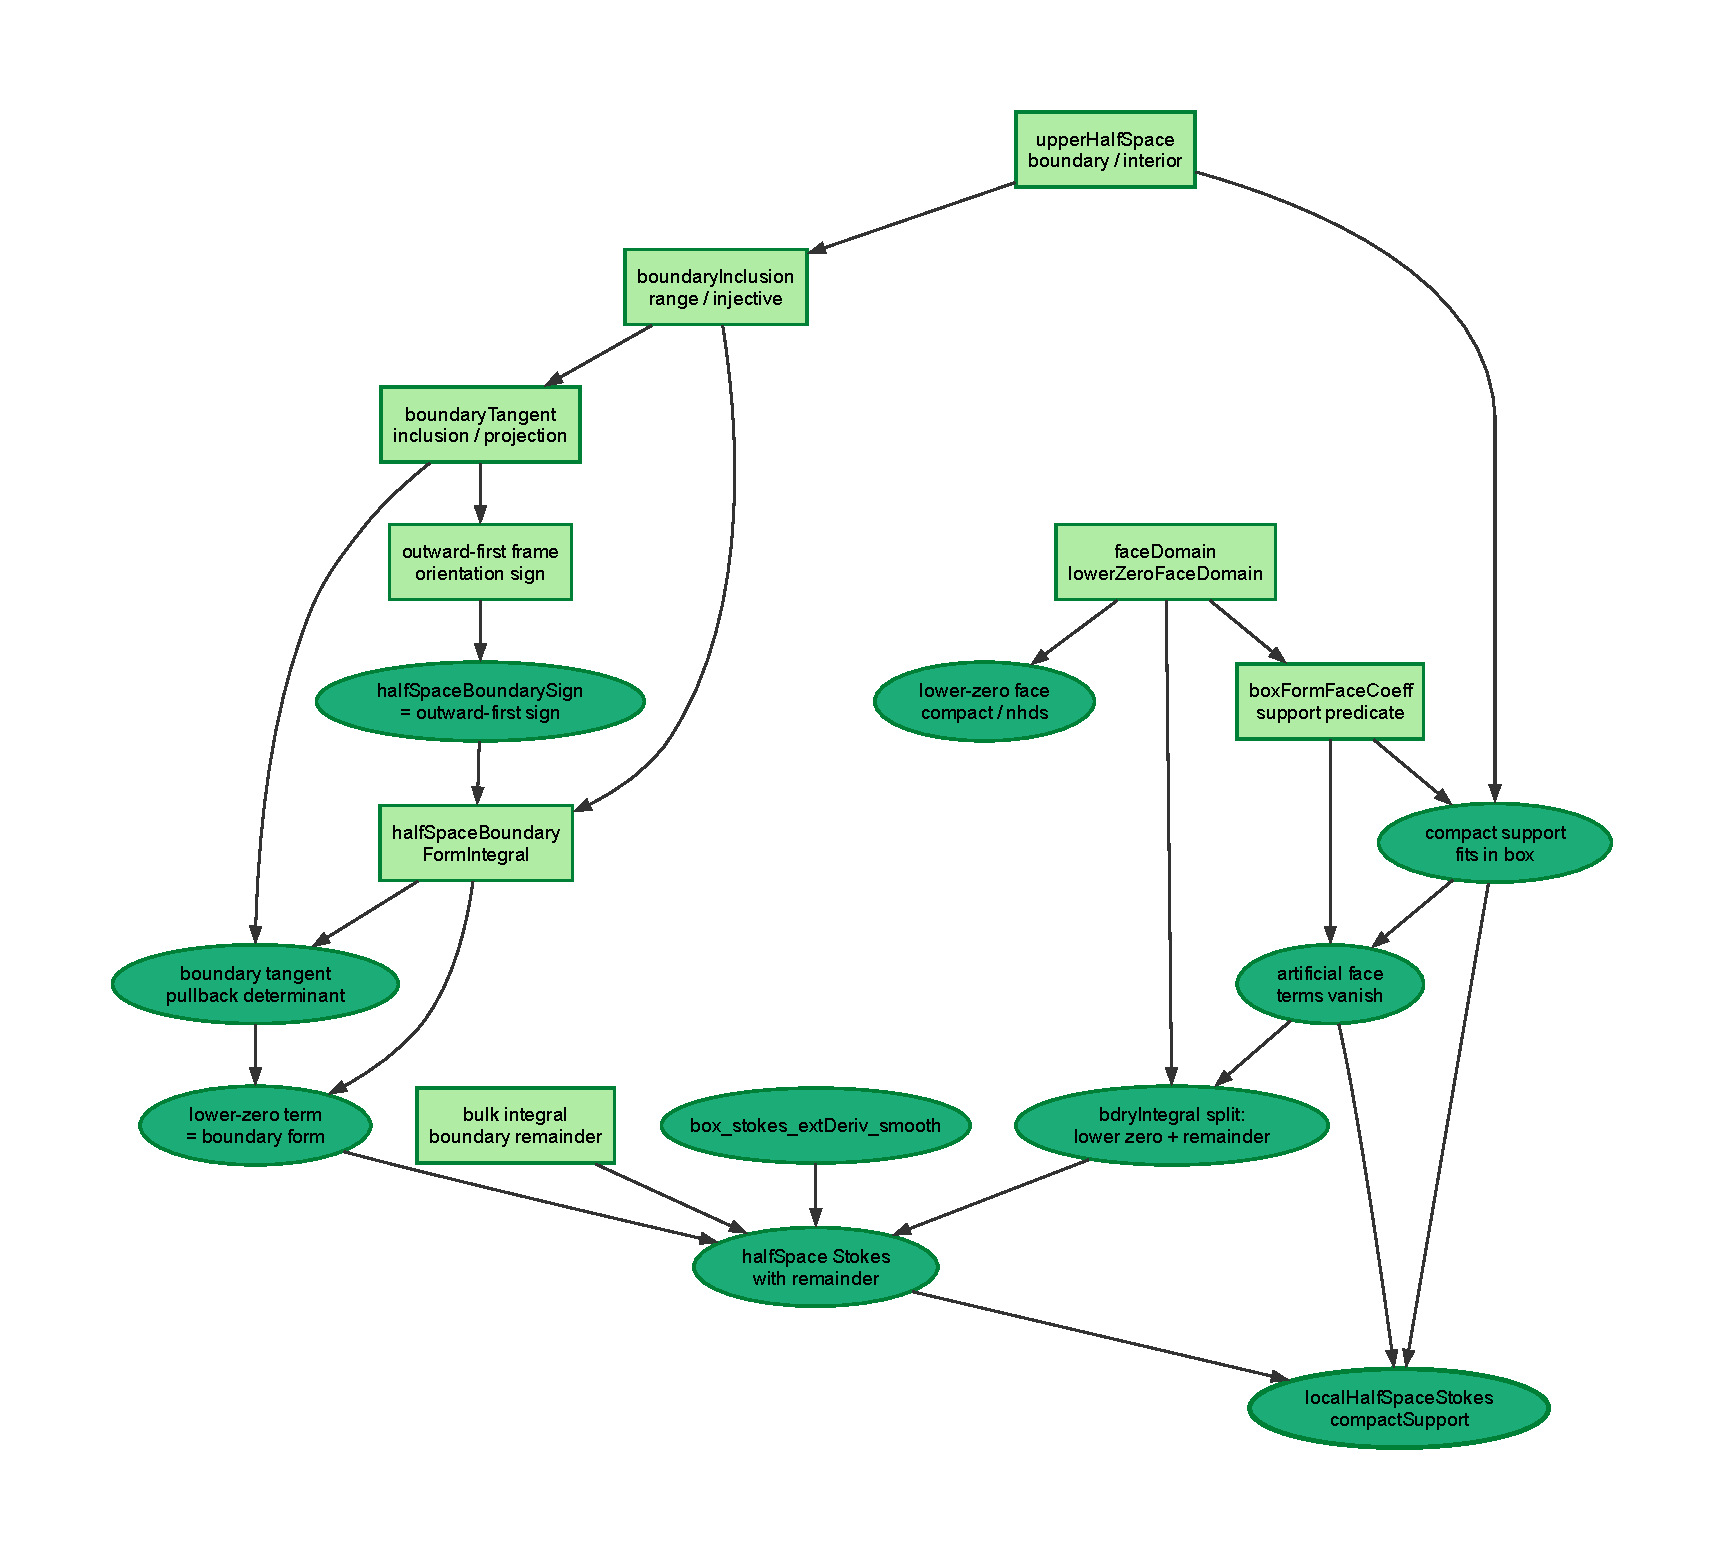
\includegraphics[width=0.90\paperheight,height=0.62\paperwidth,keepaspectratio]
      {figures/stokes-halfspace-graph.pdf}}
  \caption{Half-space local Stokes and artificial-face cancellation.}
  \label{fig:stokes_halfspace_graph}
\end{figure}
\end{landscape}

\begin{landscape}
\begin{figure}[p]
  \centering
  \noindent\makebox[\linewidth][c]{%
    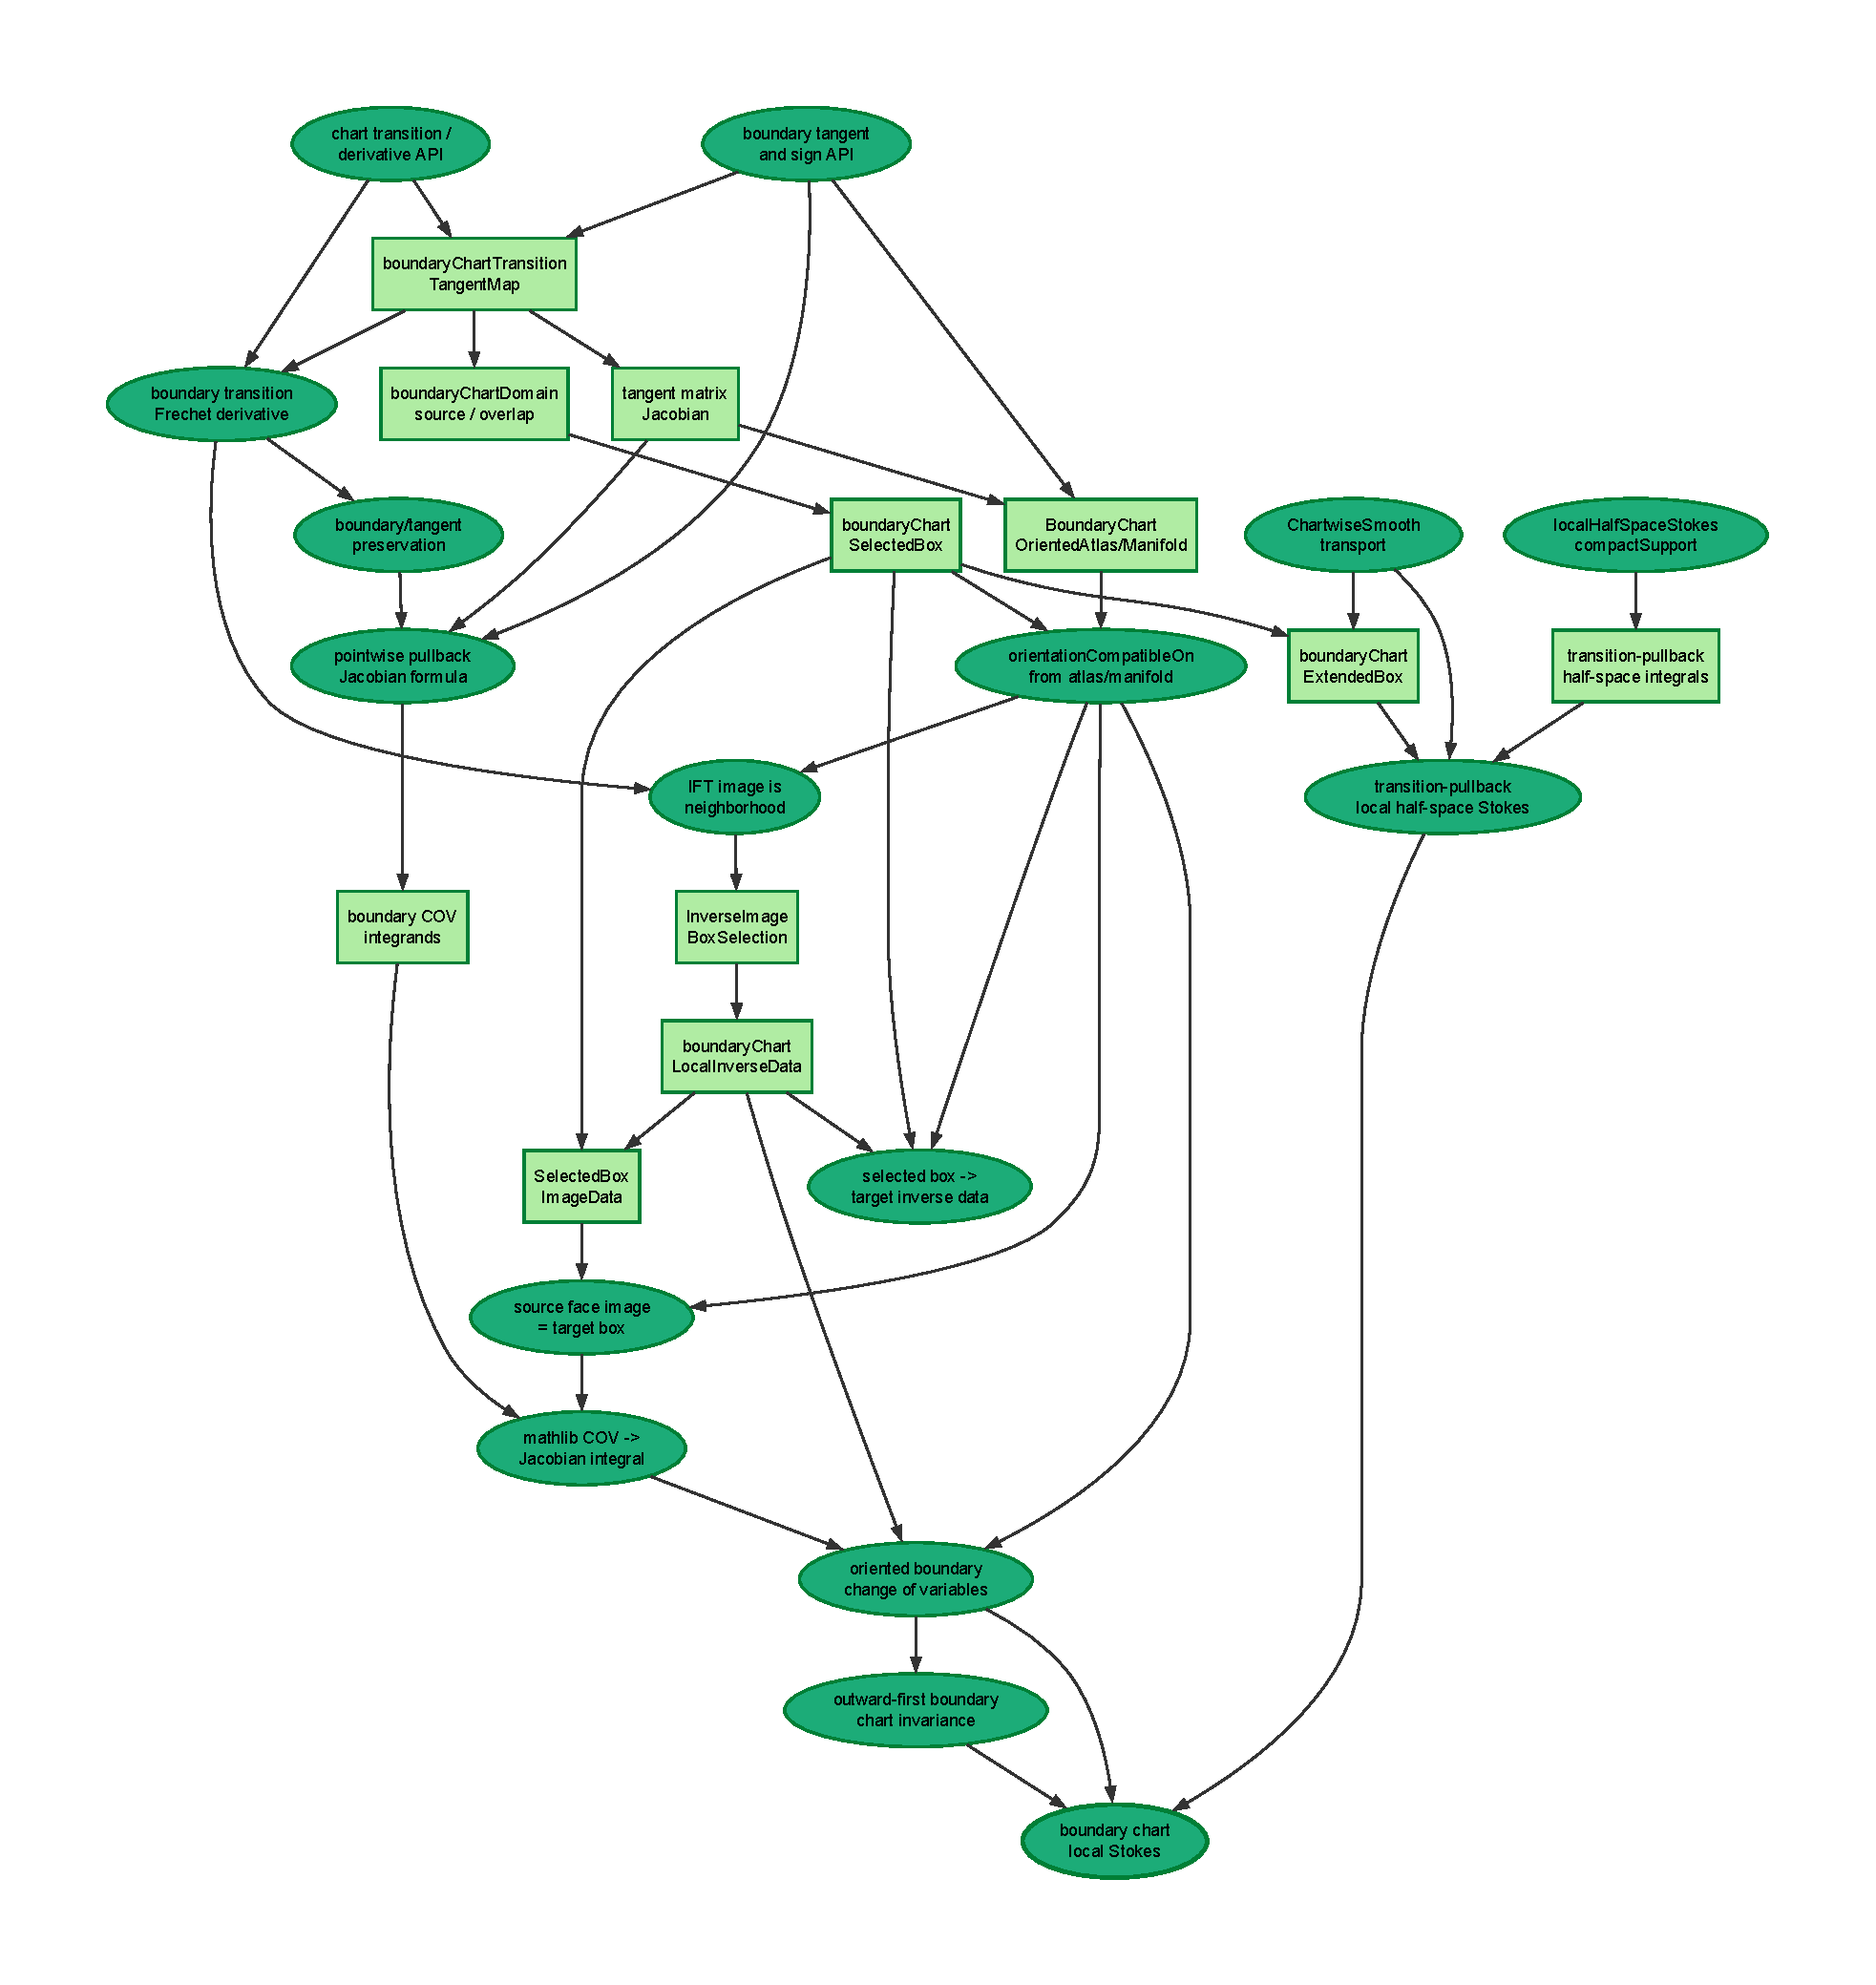
\includegraphics[width=0.90\paperheight,height=0.62\paperwidth,keepaspectratio]
      {figures/stokes-boundary-chart-graph.pdf}}
  \caption{Boundary chart change of variables and local inverse data.}
  \label{fig:stokes_boundary_chart_graph}
\end{figure}
\end{landscape}

\begin{landscape}
\begin{figure}[p]
  \centering
  \noindent\makebox[\linewidth][c]{%
    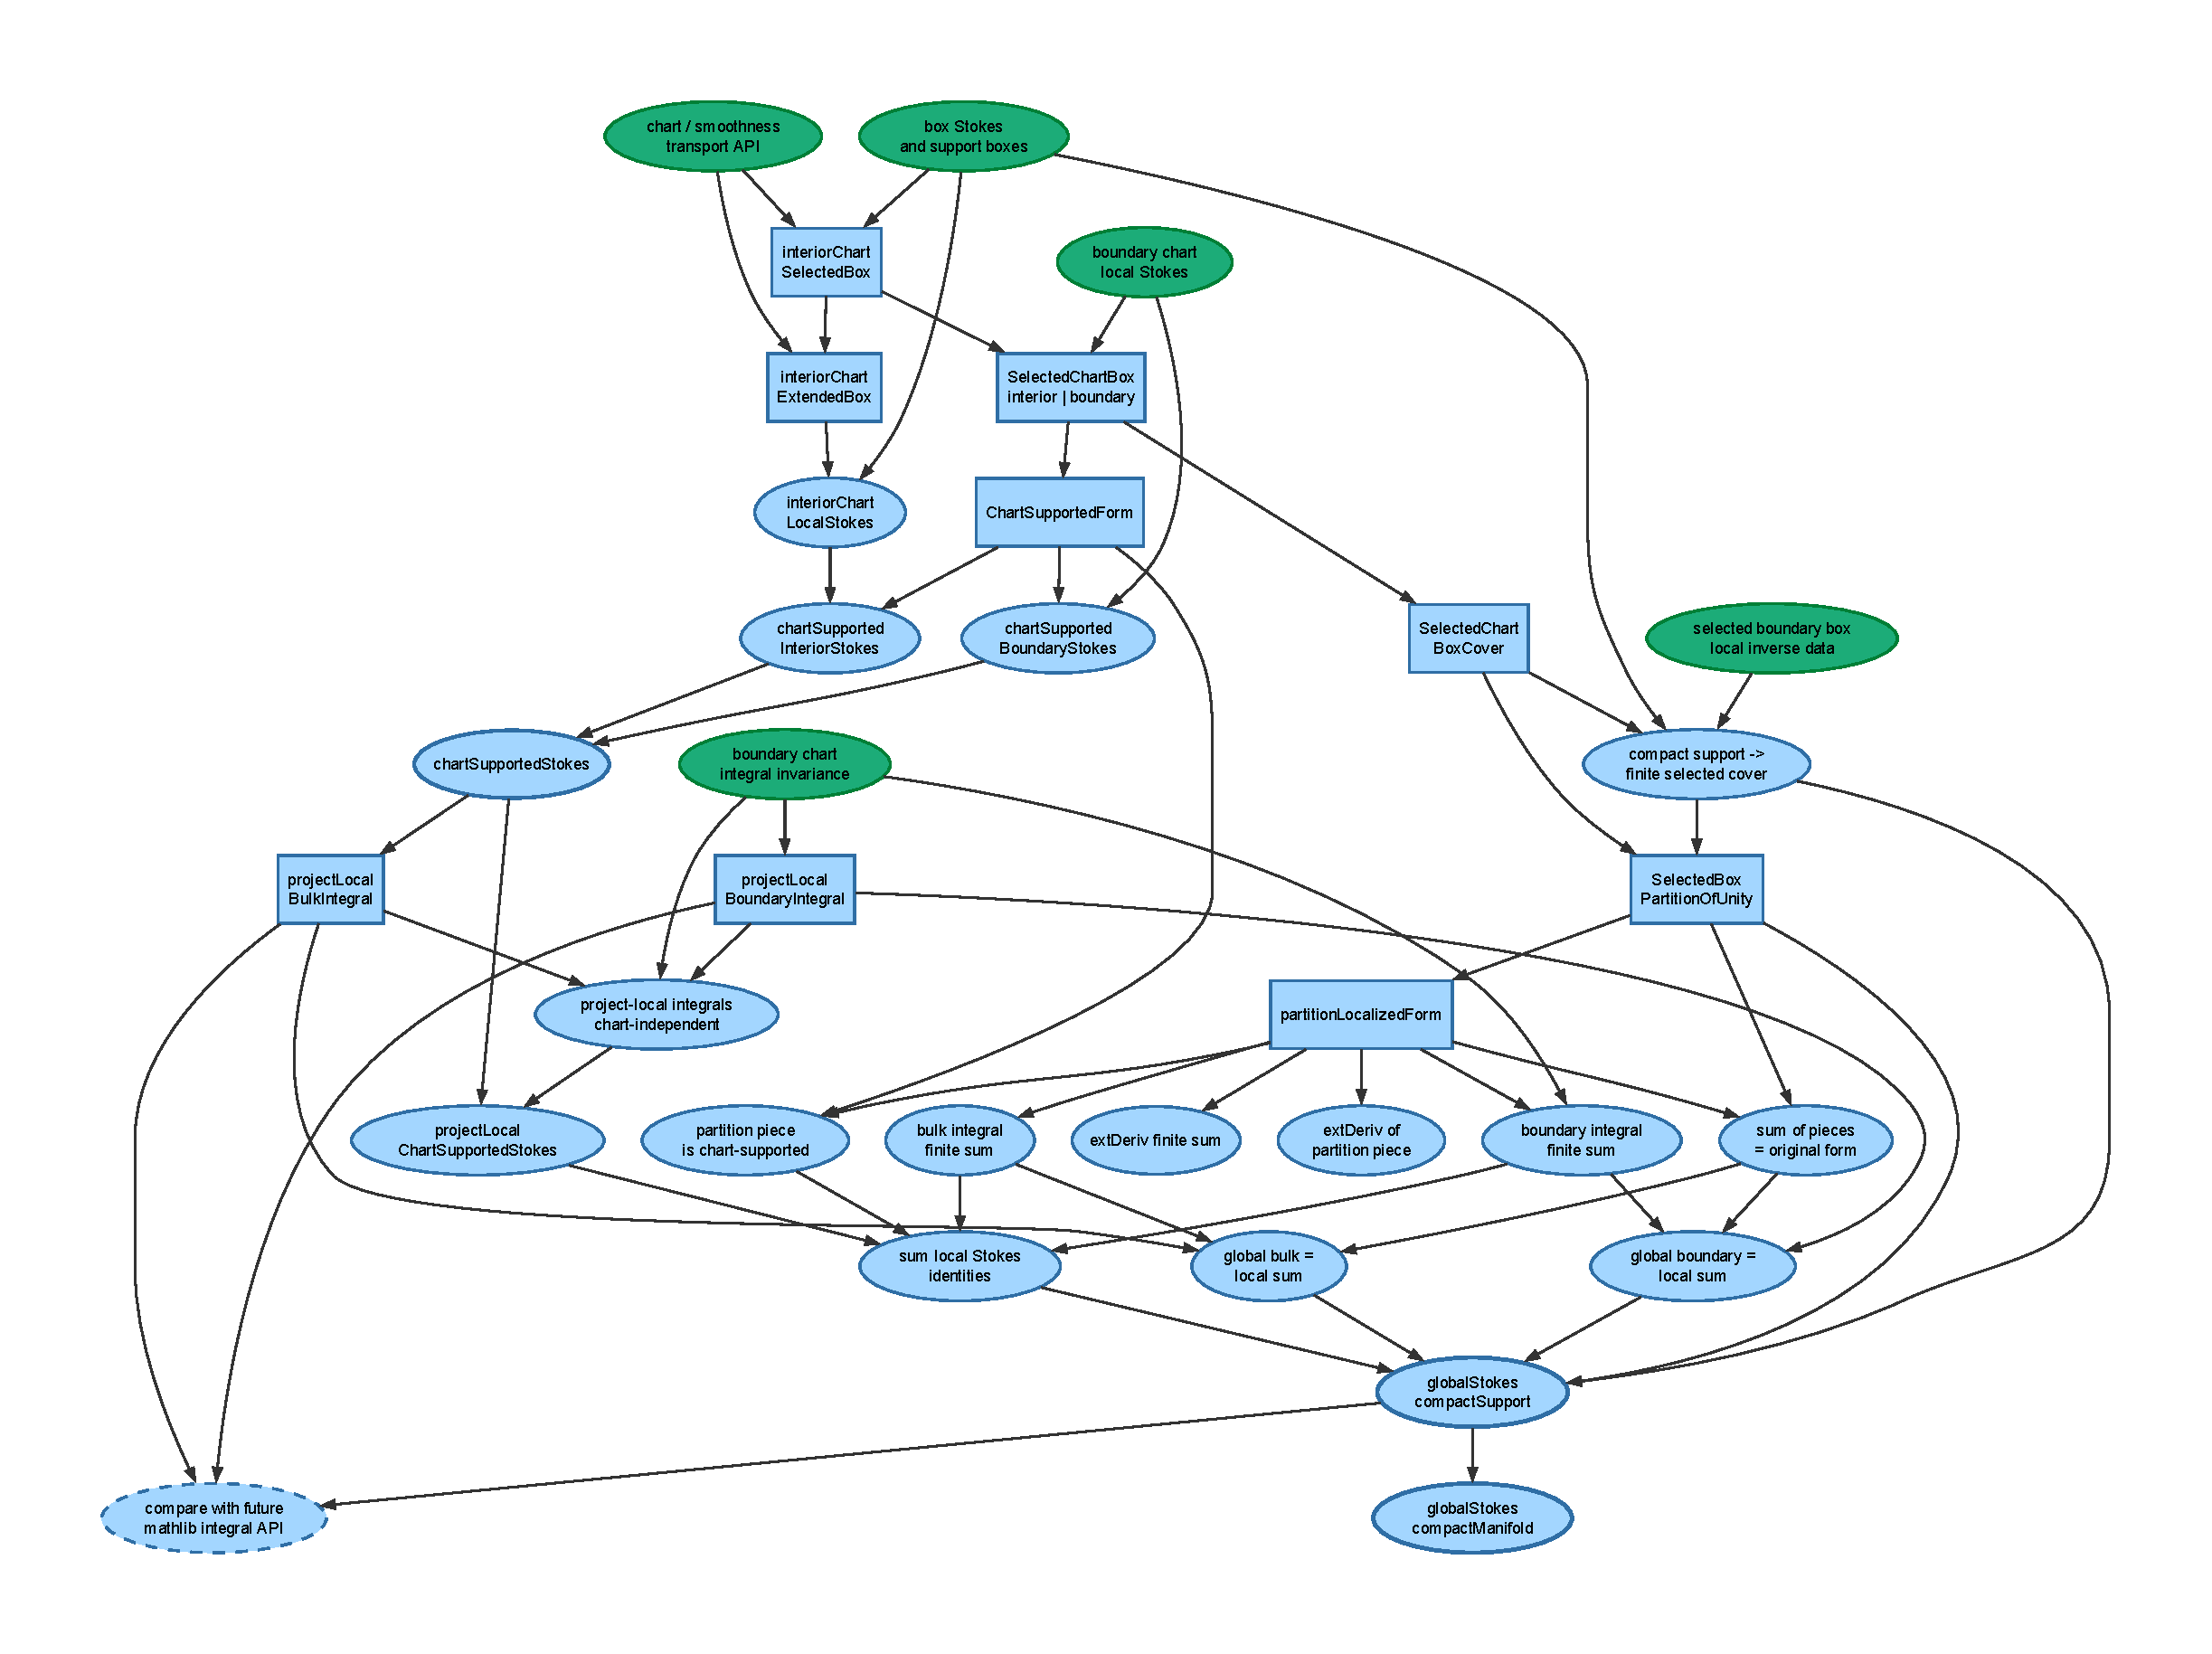
\includegraphics[width=0.90\paperheight,height=0.62\paperwidth,keepaspectratio]
      {figures/stokes-global-assembly-graph.pdf}}
  \caption{Remaining global assembly tasks.}
  \label{fig:stokes_global_graph}
\end{figure}
\end{landscape}

\begin{landscape}
\begin{figure}[p]
  \centering
  \noindent\makebox[\linewidth][c]{%
    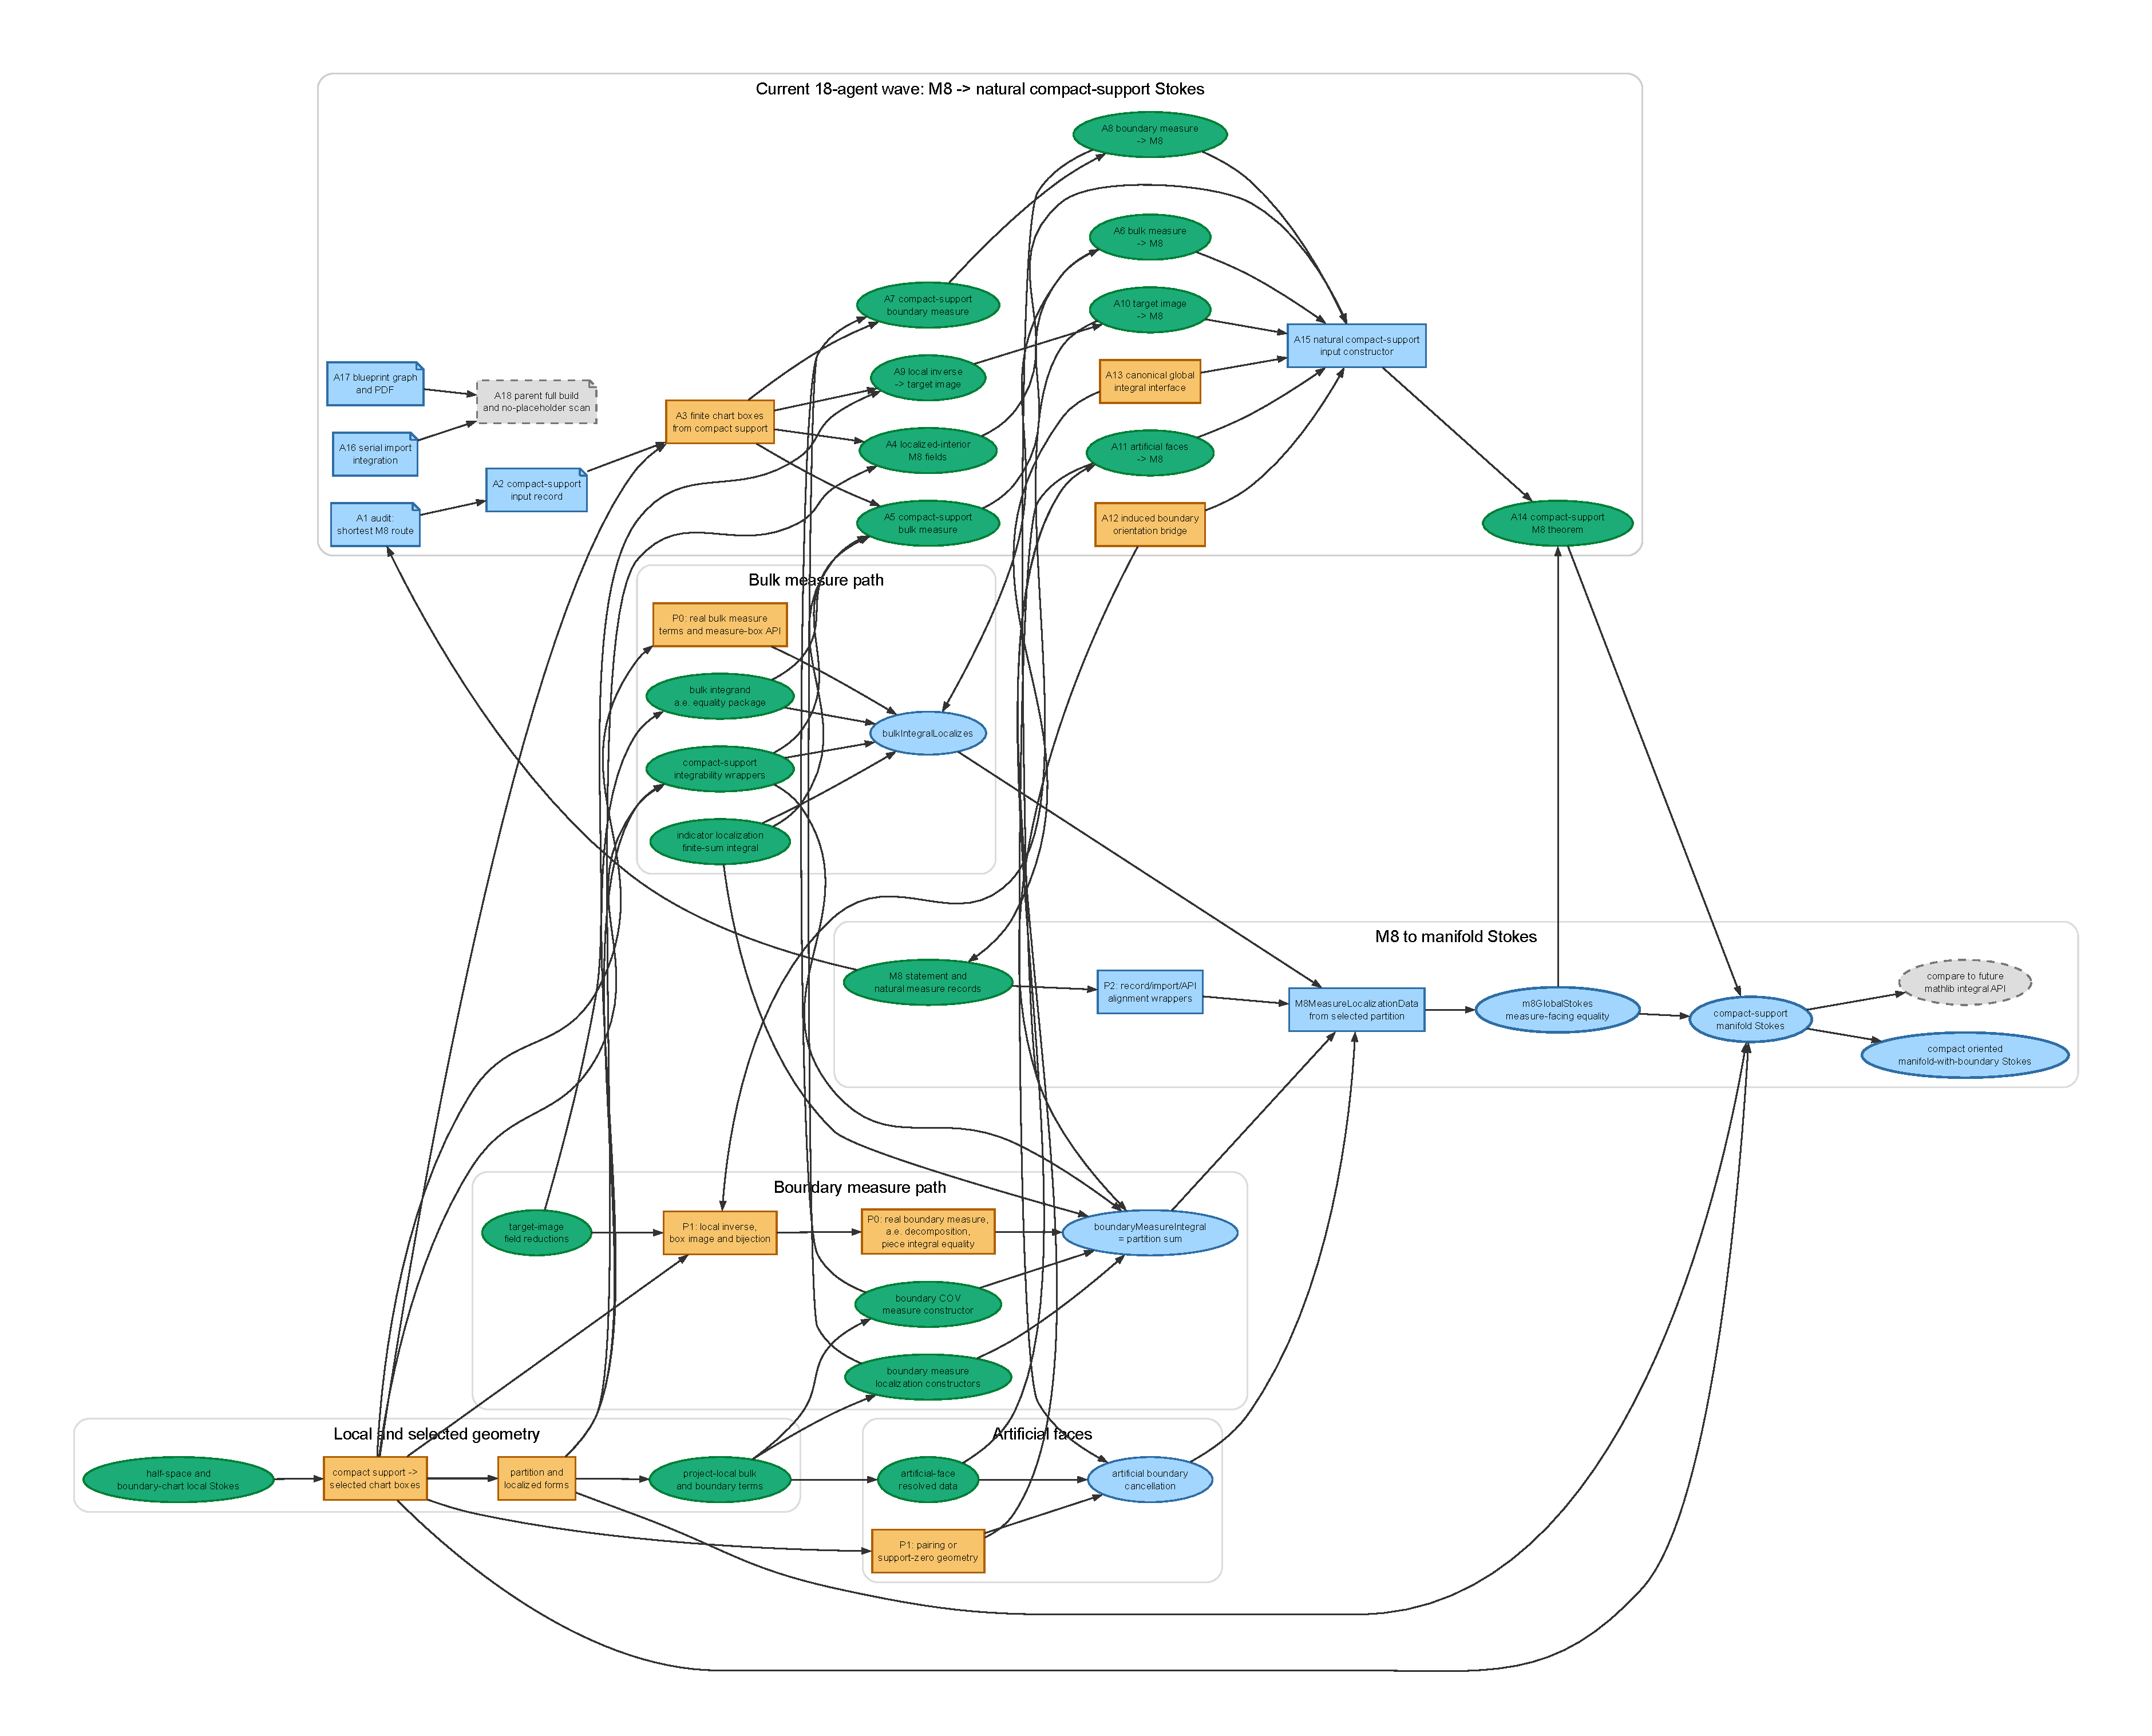
\includegraphics[width=0.90\paperheight,height=0.62\paperwidth,keepaspectratio]
      {figures/stokes-m8-measure-graph.pdf}}
  \caption{M8 measure localization, the compact-support wave, and route to manifold Stokes.}
  \label{fig:stokes_m8_measure_graph}
\end{figure}
\end{landscape}

\begin{landscape}
\begin{figure}[p]
  \centering
  \noindent\makebox[\linewidth][c]{%
    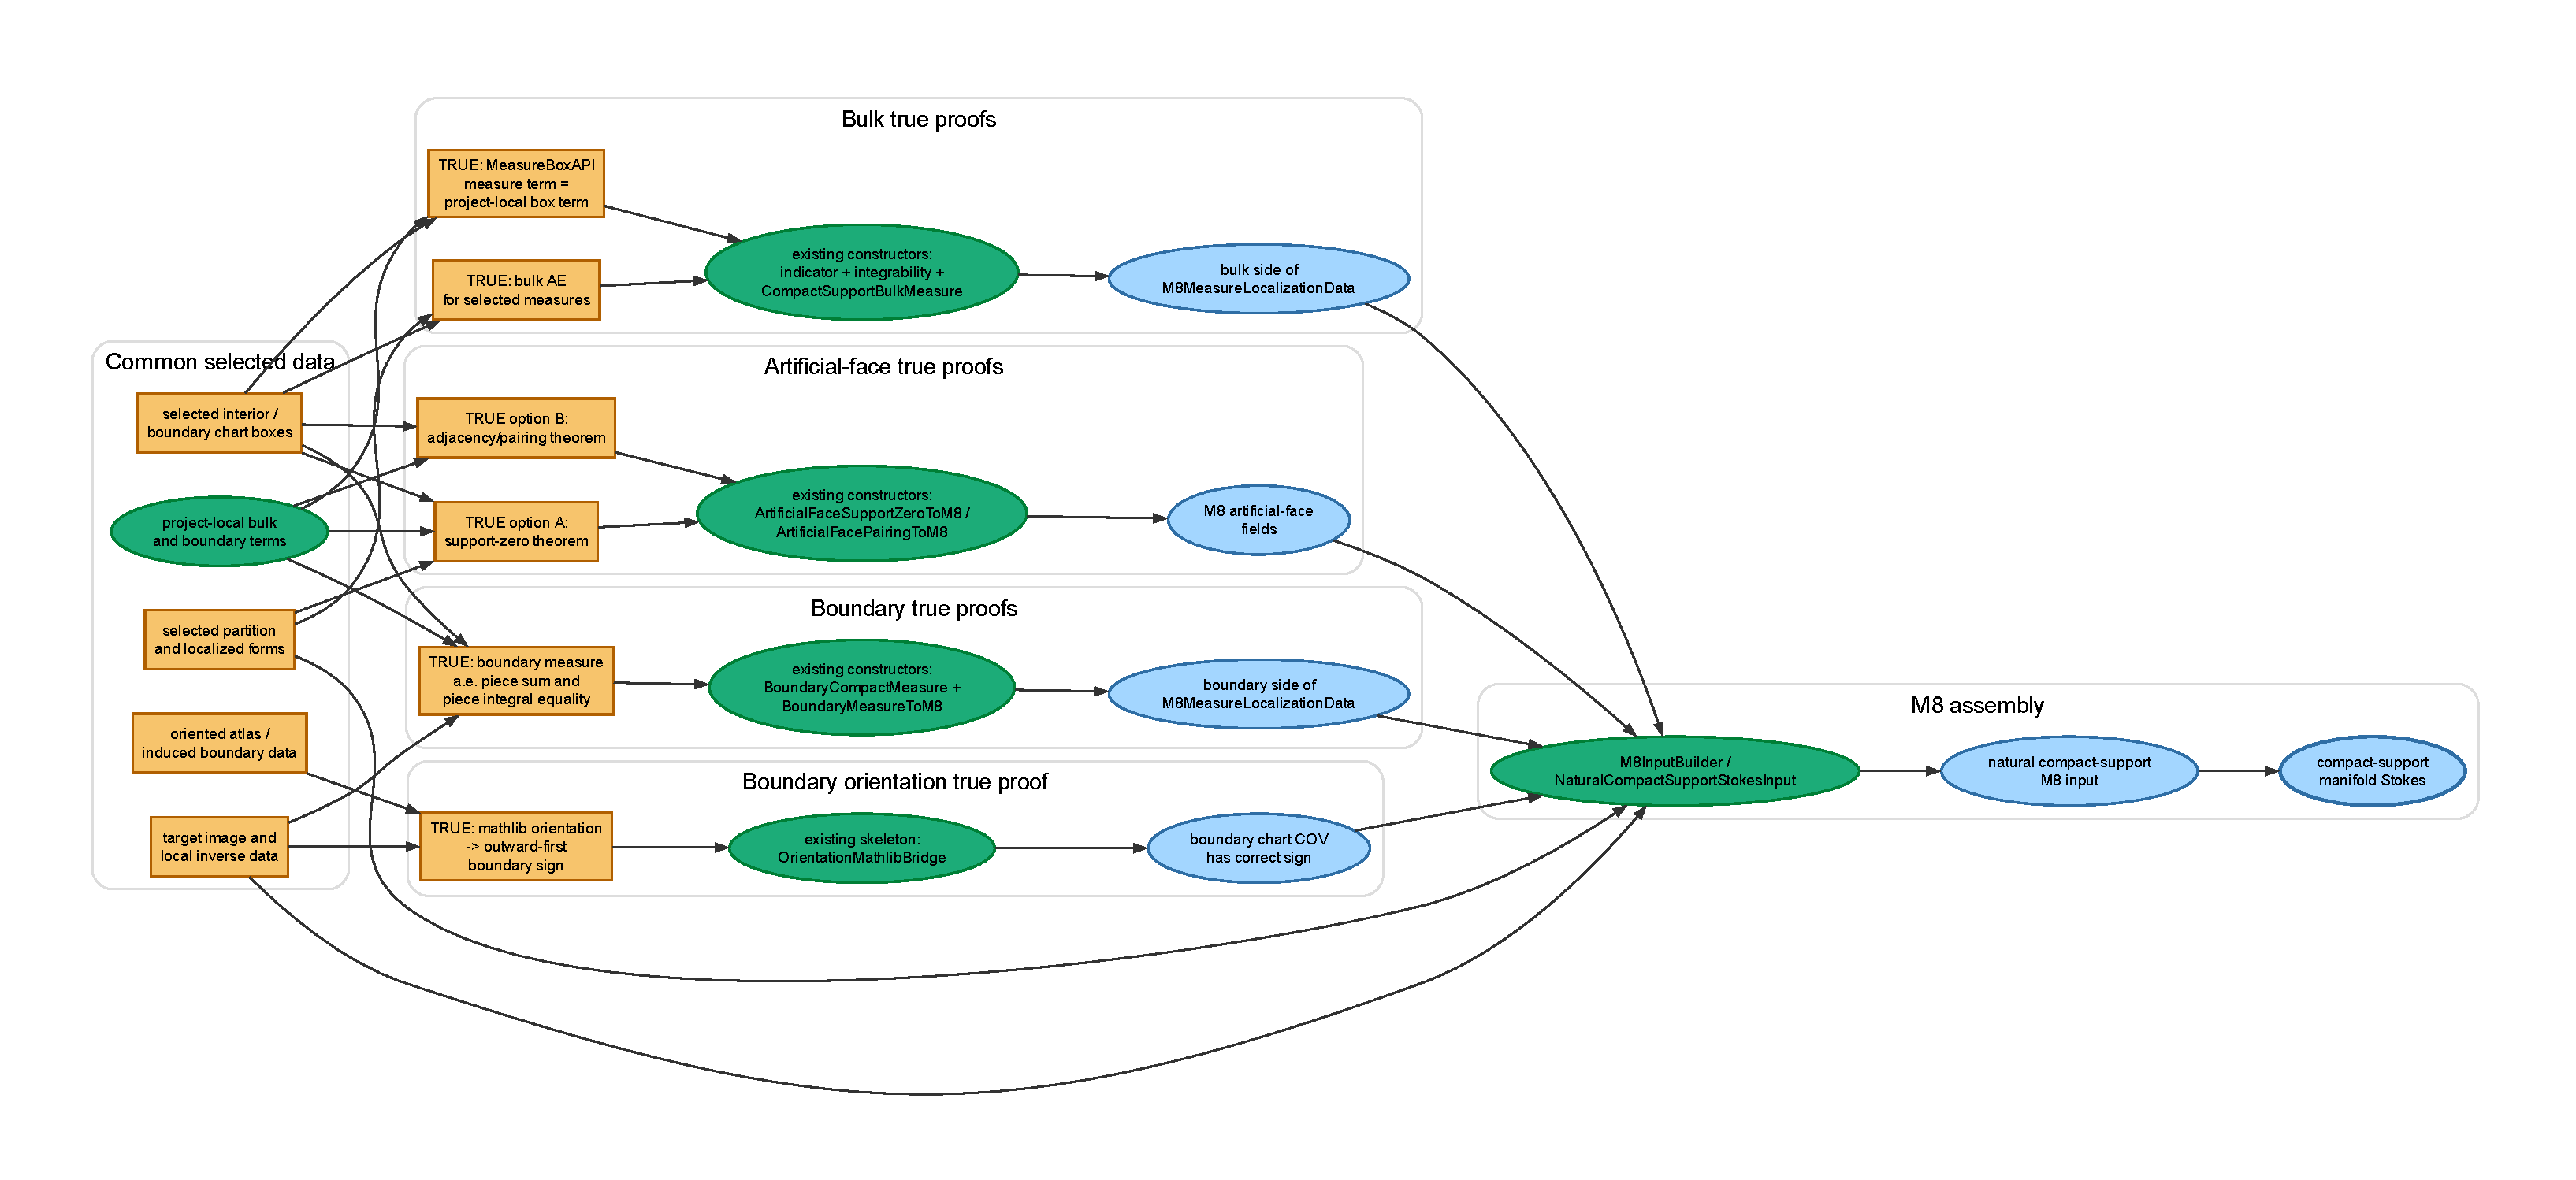
\includegraphics[width=0.88\paperheight,height=0.62\paperwidth,keepaspectratio]
      {figures/stokes-m8-proof-wave-graph.pdf}}
  \caption{Current M8 proof wave: true theorem nodes behind the compact-support route.}
  \label{fig:stokes_m8_proof_wave_graph}
\end{figure}
\end{landscape}
\clearpage

\section{Core Euclidean And Chart API}
\label{sec:core_chart_api}

\begin{definition}[Model and manifold forms]
  \label{def:model_manifold_forms}
  \lean{Stokes.ModelForm, Stokes.ManifoldForm}
  \leanok
  A model form is a topological vector-space differential form in coordinates.
  A manifold form is a fiberwise alternating map on tangent spaces.
\end{definition}

\begin{definition}[Box integral interface]
  \label{def:box_integral_interface}
  \lean{Stokes.CoordNForm, Stokes.extDerivCoord, Stokes.boxIntegral,
    Stokes.bdryIntegral}
  \leanok
  This is the thin coordinate API connecting the project to the Euclidean box
  Stokes theorem supplied by the cloned local Euclidean stack.
\end{definition}

\begin{theorem}[Box Stokes on a rectangular box]
  \label{thm:box_stokes_on_box}
  \lean{Stokes.box_stokes_on_box}
  \leanok
  \uses{def:box_integral_interface}
  The signed boundary integral of a coordinate form on an axis-aligned box is
  the integral of its coordinate exterior derivative.
\end{theorem}

\begin{theorem}[Box Stokes for mathlib forms]
  \label{thm:box_stokes_extDeriv_smooth}
  \lean{Stokes.box_stokes_extDeriv_smooth}
  \leanok
  \uses{def:model_manifold_forms, thm:box_stokes_on_box}
  The coordinate theorem is repackaged for mathlib-style differential forms and
  \texttt{extDeriv}.
\end{theorem}

\begin{definition}[Smooth singular cubes and chains]
  \label{def:smooth_singular_cube_chain}
  \lean{Stokes.SmoothSingularCube, Stokes.SingularChain,
    Stokes.singularBoundary, Stokes.integrateChain}
  \leanok
  Smooth singular cubes, their cubical faces, finite chains, and chain
  integration provide an intermediate target between boxes and manifolds.
\end{definition}

\begin{definition}[Pullback form along a cube]
  \label{def:singular_pullback_form}
  \lean{Stokes.pullbackForm, Stokes.integrateForm}
  \leanok
  \uses{def:smooth_singular_cube_chain}
  A smooth cube pulls back an ambient Euclidean form to a form on the standard
  cube, where the box theorem applies.
\end{definition}

\begin{theorem}[Exterior derivative commutes with cube pullback]
  \label{thm:singular_pullback_extDeriv}
  \lean{Stokes.singular_pullback_extDeriv}
  \leanok
  \uses{def:singular_pullback_form}
  Pulling a form back along a smooth singular cube commutes with the exterior
  derivative in the shape needed by the cubical Stokes theorem.
\end{theorem}

\begin{theorem}[Smooth singular cube Stokes]
  \label{thm:singular_cube_stokes}
  \lean{Stokes.singular_cube_stokes, Stokes.singular_cube_boundary_stokes}
  \leanok
  \uses{thm:box_stokes_extDeriv_smooth, thm:singular_pullback_extDeriv}
  Stokes holds for one smooth singular cube after expanding its oriented faces.
\end{theorem}

\begin{theorem}[Smooth singular chain Stokes]
  \label{thm:singular_chain_stokes}
  \lean{Stokes.singular_cube_chain_stokes, Stokes.singular_chain_stokes,
    Stokes.singular_boundary_boundary_zero_general}
  \leanok
  \uses{def:smooth_singular_cube_chain, thm:singular_cube_stokes}
  The cube statement extends linearly to finite chains, with boundary squared
  equal to zero.
\end{theorem}

\begin{definition}[Chart derivatives and transitions]
  \label{def:chart_derivative_transition}
  \lean{Stokes.ManifoldForm.chartInverseDeriv,
    Stokes.ManifoldForm.chartDeriv,
    Stokes.ManifoldForm.chartTransitionDeriv,
    Stokes.ManifoldForm.chartTransition,
    Stokes.ManifoldForm.chartTransitionSource}
  \leanok
  \uses{def:model_manifold_forms}
  The chart derivative API fixes the Frechet derivative maps used to express
  form pullback under coordinate changes.
\end{definition}

\begin{lemma}[Chart transition source and injectivity]
  \label{lem:chart_transition_source_inj}
  \lean{Stokes.ManifoldForm.chartTransitionSource_eq,
    Stokes.ManifoldForm.chartTransition_injOn_source,
    Stokes.ManifoldForm.chartTransition_mapsTo_extChartAt_target}
  \leanok
  \uses{def:chart_derivative_transition}
  Chart transitions are defined on the expected overlap, map into the target
  chart, and are injective on their source.
\end{lemma}

\begin{theorem}[Smoothness of chart transitions]
  \label{thm:chart_transition_smooth}
  \lean{Stokes.ManifoldForm.contDiffOn_chartTransition_source,
    Stokes.ManifoldForm.contDiffOn_chartTransition}
  \leanok
  \uses{def:chart_derivative_transition, lem:chart_transition_source_inj}
  Mathlib's manifold chart API supplies the \texttt{ContDiffOn} facts needed to
  compose chart representatives with transition maps.
\end{theorem}

\begin{theorem}[Transition derivative as Frechet derivative]
  \label{thm:chart_transition_deriv_eq}
  \lean{Stokes.ManifoldForm.chartTransitionDeriv_eq_fderivWithin}
  \leanok
  \uses{def:chart_derivative_transition}
  The concrete chart-transition derivative agrees with the Frechet derivative
  within the chart source.
\end{theorem}

\begin{theorem}[Smoothness of transition derivatives]
  \label{thm:chart_transition_deriv_smooth}
  \lean{Stokes.ManifoldForm.contDiffOn_chartTransitionDeriv_source,
    Stokes.ManifoldForm.contDiffOn_chartTransitionDeriv}
  \leanok
  \uses{thm:chart_transition_deriv_eq, thm:chart_transition_smooth}
  The derivative-valued transition map is smooth on overlaps.
\end{theorem}

\begin{definition}[Chart representative and transition pullback]
  \label{def:inchart_transition_pullback}
  \lean{Stokes.ManifoldForm.inChart,
    Stokes.ManifoldForm.transitionPullbackInChart}
  \leanok
  \uses{def:model_manifold_forms, def:chart_derivative_transition}
  A manifold form is represented in a chart, and the same representative can be
  transported through a chart transition using the transition derivative.
\end{definition}

\begin{theorem}[Chart representative compatibility]
  \label{thm:inchart_chart_transition}
  \lean{Stokes.ManifoldForm.inChart_chartTransition,
    Stokes.ManifoldForm.transitionPullbackInChart_eq_inChart}
  \leanok
  \uses{def:inchart_transition_pullback, thm:chart_transition_deriv_eq}
  On a chart overlap, the chart representative is equal to the transition
  pullback written in the source coordinates.
\end{theorem}

\begin{theorem}[Transition-pullback smoothness iff chart smoothness]
  \label{thm:transition_pullback_smooth_iff}
  \lean{Stokes.ManifoldForm.contDiffOn_inChart_of_transitionPullback,
    Stokes.ManifoldForm.contDiffOn_transitionPullbackInChart_of_contDiffOn_inChart,
    Stokes.ManifoldForm.contDiffOn_transitionPullbackInChart_iff}
  \leanok
  \uses{thm:inchart_chart_transition}
  Smoothness of the transported coordinate form is equivalent to smoothness of
  the source chart representative on the chosen overlap.
\end{theorem}

\begin{definition}[Chartwise smooth manifold form]
  \label{def:chartwise_smooth}
  \lean{Stokes.ManifoldForm.ChartwiseSmooth}
  \leanok
  \uses{def:inchart_transition_pullback}
  Chartwise smoothness packages the local smoothness hypotheses that later
  local Stokes statements consume.
\end{definition}

\begin{theorem}[Chartwise smooth transport]
  \label{thm:chartwise_smooth_transport}
  \lean{Stokes.ManifoldForm.ChartwiseSmooth.contDiffOn_inChart,
    Stokes.ManifoldForm.ChartwiseSmooth.contDiffOn_transitionPullbackInChart_of_chartAPI,
    Stokes.ManifoldForm.ChartwiseSmooth.contDiffOn_transitionPullbackInChart}
  \leanok
  \uses{def:chartwise_smooth, thm:transition_pullback_smooth_iff,
    thm:chart_transition_smooth, thm:chart_transition_deriv_smooth}
  A chartwise smooth form remains smooth after transporting it through a chart
  transition.
\end{theorem}

\section{Half-Space Local Stokes}
\label{sec:halfspace_local}

\begin{definition}[Upper half-space model]
  \label{def:upper_halfspace_model}
  \lean{Stokes.upperHalfSpace, Stokes.upperHalfSpaceBoundary,
    Stokes.upperHalfSpaceInterior}
  \leanok
  A concrete upper half-space in \(\R^{n+1}\) fixes the local boundary model.
\end{definition}

\begin{definition}[Boundary inclusion and tangent maps]
  \label{def:boundary_inclusion_tangent}
  \lean{Stokes.boundaryInclusion, Stokes.range_boundaryInclusion,
    Stokes.boundaryInclusion_injective, Stokes.boundaryTangentInclusion,
    Stokes.boundaryTangentProjection}
  \leanok
  \uses{def:upper_halfspace_model}
  The boundary hyperplane is identified with \(\R^n\), together with the
  tangent inclusion and projection used by boundary forms.
\end{definition}

\begin{definition}[Outward-first frame and sign]
  \label{def:outward_first_frame_sign}
  \lean{Stokes.outwardNormal, Stokes.outwardFirstBoundaryFrame,
    Stokes.outwardFirstBoundaryMatrix,
    Stokes.det_outwardFirstBoundaryMatrix,
    Stokes.outwardFirstBoundaryOrientationSign,
    Stokes.halfSpaceBoundarySign,
    Stokes.halfSpaceBoundarySign_eq_outwardFirstBoundaryOrientationSign}
  \leanok
  \uses{def:boundary_inclusion_tangent}
  The lower face of the box has the same sign as the outward-normal-first
  boundary orientation.
\end{definition}

\begin{definition}[Box faces and face coefficients]
  \label{def:box_faces_coefficients}
  \lean{Stokes.faceDomain, Stokes.lowerZeroFaceDomain,
    Stokes.boxUpperFormFaceIntegral, Stokes.boxLowerFormFaceIntegral,
    Stokes.boxFormFaceCoeff, Stokes.boxFaceMap,
    Stokes.boxFaceCoeffTSupportInHalfSpaceBox}
  \leanok
  \uses{thm:box_stokes_extDeriv_smooth}
  The box boundary integral is decomposed into the true boundary face and the
  artificial faces introduced by localizing to a box.
\end{definition}

\begin{lemma}[Compact support fits in a half-space box]
  \label{lem:halfspace_support_box_selection}
  \lean{Stokes.exists_halfSpaceSupportBox_of_isCompact,
    Stokes.boxFaceCoeffTSupportInHalfSpaceBox_of_tsupport_subset,
    Stokes.boxFormFaceCoeff_tsupport_subset}
  \leanok
  \uses{def:upper_halfspace_model, def:box_faces_coefficients}
  Compact support contained in the half-space can be enclosed in a box whose
  artificial faces miss the support.
\end{lemma}

\begin{lemma}[Boundary face domain compactness]
  \label{lem:lower_zero_face_domain_selection}
  \lean{Stokes.isCompact_lowerZeroFaceDomain,
    Stokes.exists_lowerZeroFaceDomain_of_isCompact,
    Stokes.lowerZeroFaceDomain_mem_nhds_of_lt,
    Stokes.exists_lowerZeroFaceDomain_subset_of_mem_nhds}
  \leanok
  \uses{def:box_faces_coefficients}
  A boundary face domain is compact and can be shrunk or selected inside a
  prescribed neighborhood.
\end{lemma}

\begin{theorem}[Artificial face terms vanish]
  \label{thm:artificial_faces_vanish}
  \lean{Stokes.boxRemainingFormFaceTerms_eq_zero_of_face_cancellation,
    Stokes.boxRemainingFormFaceTerms_eq_zero_of_support_disjoint,
    Stokes.boxRemainingFormFaceTerms_eq_zero_of_tsupport_subset_halfSpaceSupportBox,
    Stokes.boxArtificialFaces_tsupport_disjoint_of_subset_halfSpaceSupportBox}
  \leanok
  \uses{def:box_faces_coefficients, lem:halfspace_support_box_selection}
  If the form is supported in the selected half-space box, every artificial
  face contribution is zero.
\end{theorem}

\begin{theorem}[Boundary integral splits into true face plus remainder]
  \label{thm:box_boundary_split}
  \lean{Stokes.boxRemainingCoordFaceTerms_toCoordNForm,
    Stokes.bdryIntegral_eq_lowerZero_add_remaining}
  \leanok
  \uses{def:box_faces_coefficients, thm:artificial_faces_vanish}
  The box boundary integral separates the lower-zero face from all remaining
  artificial faces.
\end{theorem}

\begin{definition}[Half-space boundary integral]
  \label{def:halfspace_boundary_integral}
  \lean{Stokes.halfSpaceBoundaryCoordTerm,
    Stokes.halfSpaceBoundaryFormIntegral,
    Stokes.outwardFirstHalfSpaceBoundaryFormIntegral}
  \leanok
  \uses{def:outward_first_frame_sign, def:boundary_inclusion_tangent}
  The true boundary term is written as an integral over the boundary hyperplane
  using the outward-first sign convention.
\end{definition}

\begin{theorem}[Boundary tangent pullback determinant formula]
  \label{thm:boundary_tangent_pullback_det}
  \lean{Stokes.boundaryTangentPullbackForm,
    Stokes.boundaryTangentPullbackForm_comp_apply_basisFun_eq_det_mul,
    Stokes.ambientBoundaryForm_tangentMap_eq_det_mul}
  \leanok
  \uses{def:boundary_inclusion_tangent, def:halfspace_boundary_integral}
  Pulling a top-degree boundary form through a linear tangent map multiplies
  the coordinate coefficient by the determinant.
\end{theorem}

\begin{theorem}[Lower-zero face equals boundary form]
  \label{thm:lower_zero_face_eq_boundary_form}
  \lean{Stokes.lowerZero_toCoordNForm_eq_boundaryForm,
    Stokes.halfSpaceBoundaryCoordTerm_toCoordNForm,
    Stokes.boxLowerZeroCoordFaceTerm_toCoordNForm_eq_halfSpaceBoundaryFormTerm}
  \leanok
  \uses{def:halfspace_boundary_integral, thm:boundary_tangent_pullback_det}
  The lower-zero face coefficient extracted from the box is exactly the
  half-space boundary form coefficient.
\end{theorem}

\begin{definition}[Half-space local bulk and remainder]
  \label{def:halfspace_bulk_remainder}
  \lean{Stokes.standardTopFrame, Stokes.halfSpaceLocalBulkIntegral,
    Stokes.halfSpaceLocalBoundaryRemainder}
  \leanok
  \uses{def:halfspace_boundary_integral, def:box_faces_coefficients}
  The local theorem is stated as a bulk integral equals a boundary integral plus
  a remainder from artificial faces.
\end{definition}

\begin{theorem}[Half-space Stokes with remainder]
  \label{thm:halfspace_stokes_with_remainder}
  \lean{Stokes.box_stokes_extDeriv_contDiffOn_isOpen,
    Stokes.halfSpaceLocalStokes_with_remainder,
    Stokes.halfSpaceLocalStokes_with_remainder_of_contDiffOn_isOpen}
  \leanok
  \uses{thm:box_stokes_extDeriv_smooth, thm:box_boundary_split,
    thm:lower_zero_face_eq_boundary_form, def:halfspace_bulk_remainder}
  The box theorem gives local half-space Stokes before canceling artificial
  faces.
\end{theorem}

\begin{theorem}[Half-space Stokes with compact support]
  \label{thm:halfspace_stokes_compact_support}
  \lean{Stokes.halfSpaceLocalBoundaryRemainder_eq_zero_of_tsupport_subset_halfSpaceSupportBox,
    Stokes.halfSpaceLocalStokes_compactSupport,
    Stokes.halfSpaceLocalStokes_compactSupport_of_contDiffOn_isOpen,
    Stokes.localHalfSpaceStokes_compactSupport,
    Stokes.localHalfSpaceStokes_compactSupport_of_contDiffOn_isOpen}
  \leanok
  \uses{thm:halfspace_stokes_with_remainder, thm:artificial_faces_vanish}
  Once support is contained in the selected half-space box, the remainder
  vanishes and the local half-space Stokes theorem is obtained.
\end{theorem}

\section{Boundary Chart Change}
\label{sec:boundary_chart_change}

\begin{definition}[Boundary chart transition]
  \label{def:boundary_chart_transition}
  \lean{Stokes.boundaryChartTransition,
    Stokes.boundaryChartTransition_apply,
    Stokes.boundaryChartTransitionTangentMap,
    Stokes.boundaryChartTransitionTangentMap_apply}
  \leanok
  \uses{def:chart_derivative_transition, def:boundary_inclusion_tangent}
  A boundary chart transition is the tangential coordinate map induced by an
  ambient chart transition preserving the boundary hyperplane.
\end{definition}

\begin{theorem}[Boundary chart transition derivative]
  \label{thm:boundary_chart_transition_derivative}
  \lean{Stokes.boundaryChartTransition_hasFDerivWithinAt,
    Stokes.boundaryChartTransition_hasFDerivWithinAt_of_selectedBox,
    Stokes.boundaryChartTransition_hasFDerivAt_of_selectedBox_mem_nhds}
  \leanok
  \uses{def:boundary_chart_transition, thm:chart_transition_deriv_eq}
  The Frechet derivative of the boundary chart transition is the tangential map
  obtained by restricting the ambient chart derivative.
\end{theorem}

\begin{definition}[Boundary Jacobian]
  \label{def:boundary_chart_jacobian}
  \lean{Stokes.boundaryChartTransitionMatrix,
    Stokes.boundaryChartTransitionMatrix_det_eq_linearMap_det,
    Stokes.boundaryChartTransitionJacobian}
  \leanok
  \uses{def:boundary_chart_transition}
  The tangential derivative is converted to a matrix determinant for the
  Euclidean change-of-variables theorem.
\end{definition}

\begin{theorem}[Boundary preservation and tangent preservation]
  \label{thm:boundary_tangent_preservation}
  \lean{Stokes.boundaryChartTransitionPreservesBoundaryAt,
    Stokes.boundaryChartTransitionPreservesBoundaryAt_of_zero,
    Stokes.boundaryChartTransitionDerivPreservesTangentAt,
    Stokes.boundaryChartTransitionDerivPreservesTangentAt_of_normal_zero}
  \leanok
  \uses{def:boundary_chart_transition, thm:boundary_chart_transition_derivative}
  The chart transition and its derivative preserve the boundary tangent
  hyperplane under the expected coordinate zero hypotheses.
\end{theorem}

\begin{theorem}[Pointwise boundary pullback determinant]
  \label{thm:boundary_pointwise_pullback_det}
  \lean{Stokes.boundaryChartTransition_pointwise_pullback_det}
  \leanok
  \uses{def:boundary_chart_jacobian, thm:boundary_tangent_pullback_det,
    thm:boundary_tangent_preservation}
  The boundary integrand after chart change is the original boundary integrand
  multiplied by the tangential Jacobian.
\end{theorem}

\begin{definition}[Boundary chart domain]
  \label{def:boundary_chart_domain}
  \lean{Stokes.boundaryChartDomain,
    Stokes.boundaryChartTransitionBoundarySource,
    Stokes.mem_boundaryChartTransitionBoundarySource_iff,
    Stokes.boundaryChartDomain_eq_chartTransitionSource,
    Stokes.boundaryChartDomain_subset_target,
    Stokes.boundaryChartDomain_subset_overlap}
  \leanok
  \uses{def:boundary_chart_transition, lem:chart_transition_source_inj}
  The boundary transition source is related to the ambient chart-transition
  source and overlap.
\end{definition}

\begin{definition}[Selected boundary chart box]
  \label{def:boundary_chart_selected_box}
  \lean{Stokes.boundaryChartSelectedBox,
    Stokes.boundaryChartSelectedBox.mk_of_subsets,
    Stokes.boundaryChartSelectedBox.Icc_subset_domain,
    Stokes.boundaryChartSelectedBox.tsupport_subset,
    Stokes.boundaryChartSelectedBox.boundaryFace_subset_overlap,
    Stokes.boundaryChartSelectedBox.boundaryFace_subset_range}
  \leanok
  \uses{def:boundary_chart_domain, lem:halfspace_support_box_selection}
  A selected source box records the local domain, support containment, and
  boundary-face overlap facts needed by local Stokes.
\end{definition}

\begin{definition}[Extended boundary chart box]
  \label{def:boundary_chart_extended_box}
  \lean{Stokes.boundaryChartExtendedBox,
    Stokes.boundaryChartExtendedBox.mk,
    Stokes.boundaryChartExtendedBox.selectedBox,
    Stokes.boundaryChartExtendedBox.exists_smooth_nhds,
    Stokes.boundaryChartExtendedBox.boundaryFace_subset_overlap}
  \leanok
  \uses{def:boundary_chart_selected_box, thm:chartwise_smooth_transport}
  The selected box is strengthened with a neighborhood where the transported
  chart form has \texttt{ContDiffOn} smoothness.
\end{definition}

\begin{definition}[Boundary chart oriented atlas]
  \label{def:boundary_chart_oriented_atlas}
  \lean{Stokes.boundaryChartOrientationCompatibleOn,
    Stokes.boundaryChartPreservesOrientationOn,
    Stokes.boundaryChartOrientationCompatibleOn_of_preservesOrientationOn,
    Stokes.BoundaryChartOrientedAtlas,
    Stokes.BoundaryChartOrientedManifold}
  \leanok
  \uses{def:boundary_chart_jacobian, def:outward_first_frame_sign}
  This is the local orientation bridge: oriented boundary charts have positive
  tangential Jacobian on the relevant boundary box.
\end{definition}

\begin{theorem}[Orientation compatibility from atlas data]
  \label{thm:boundary_orientation_from_atlas}
  \lean{Stokes.BoundaryChartOrientedAtlas.orientationCompatibleOn_selectedBox,
    Stokes.BoundaryChartOrientedAtlas.boundaryChartOrientationCompatibleOn_of_orientedAtlas,
    Stokes.BoundaryChartOrientedManifold.boundaryChartOrientationCompatibleOn_of_orientedManifold,
    Stokes.BoundaryChartOrientedManifold.boundaryChartOrientationCompatibleOn_selectedBox_of_orientedManifold}
  \leanok
  \uses{def:boundary_chart_selected_box, def:boundary_chart_oriented_atlas}
  The explicit positive-Jacobian condition can be obtained from the chosen
  oriented atlas or oriented-manifold class.
\end{theorem}

\begin{theorem}[Local image is a neighborhood]
  \label{thm:boundary_transition_open_image}
  \lean{Stokes.boundaryChartTransitionTangentMap_range_eq_top_of_jacobian_ne_zero,
    Stokes.boundaryChartTransitionTangentMap_range_eq_top_of_orientationCompatibleOn,
    Stokes.boundaryChartTransition_hasStrictFDerivAt_of_contDiffAt_hasFDerivAt,
    Stokes.boundaryChartTransition_image_mem_nhds_of_hasStrictFDerivAt_surj,
    Stokes.boundaryChartTransition_image_mem_nhds_of_hasStrictFDerivAt_orientationCompatibleOn}
  \leanok
  \uses{thm:boundary_chart_transition_derivative, thm:boundary_orientation_from_atlas}
  The inverse function theorem gives that the boundary chart transition maps a
  small source neighborhood onto a target neighborhood.
\end{theorem}

\begin{definition}[Boundary local inverse data]
  \label{def:boundary_local_inverse_data}
  \lean{Stokes.boundaryChartInverseImageBoxSelection,
    Stokes.boundaryChartLocalInverseData,
    Stokes.boundaryChartLocalInverseData.of_inverseImageBoxSelection,
    Stokes.boundaryChartLocalInverseData.surjOn}
  \leanok
  \uses{lem:lower_zero_face_domain_selection, thm:boundary_transition_open_image}
  Local inverse data packages a target boundary box and a right inverse into the
  source boundary box.
\end{definition}

\begin{theorem}[Selected source box gives target inverse data]
  \label{thm:exists_boundary_local_inverse_data}
  \lean{Stokes.exists_boundaryChartInverseImageBoxSelection_of_selectedBox_orientedAtlas,
    Stokes.exists_boundaryChartInverseImageBoxSelection_of_selectedBox_orientedManifold,
    Stokes.exists_boundaryChartLocalInverseData_of_selectedBox_orientedAtlas_lt,
    Stokes.exists_boundaryChartLocalInverseData_of_selectedBox_orientedManifold_lt}
  \leanok
  \uses{def:boundary_chart_selected_box, def:boundary_local_inverse_data,
    thm:boundary_orientation_from_atlas}
  A selected source boundary box, an interior boundary point, and oriented atlas
  data produce the target box and local inverse data needed for chart change.
\end{theorem}

\begin{definition}[Boundary selected box image data]
  \label{def:boundary_selected_box_image_data}
  \lean{Stokes.boundaryChartSelectedBoxImageData,
    Stokes.boundaryChartSelectedBoxImageData.mapsTo,
    Stokes.boundaryChartSelectedBoxImageData.surjOn,
    Stokes.boundaryChartSelectedBoxImageData_of_mapsTo_localInverseData,
    Stokes.boundaryChartSelectedBoxImageData_of_compactImage_localInverseData}
  \leanok
  \uses{def:boundary_chart_selected_box, def:boundary_local_inverse_data}
  Image data is the version of local inverse information consumed by the
  integral invariance theorems.
\end{definition}

\begin{theorem}[Selected boundary box image equality]
  \label{thm:boundary_selected_box_image_eq}
  \lean{Stokes.boundaryChartTransition_image_eq_lowerZeroFaceDomain_of_selectedBox_orientedAtlas,
    Stokes.boundaryChartTransition_image_eq_lowerZeroFaceDomain_of_orientedAtlas_imageData,
    Stokes.boundaryChartTransition_image_eq_lowerZeroFaceDomain_of_selectedBox_orientedManifold,
    Stokes.boundaryChartTransition_image_eq_lowerZeroFaceDomain_of_orientedManifold_imageData}
  \leanok
  \uses{def:boundary_selected_box_image_data, thm:boundary_orientation_from_atlas}
  The boundary chart transition maps the source boundary face exactly to the
  chosen target boundary box.
\end{theorem}

\begin{theorem}[Boundary change of variables]
  \label{thm:boundary_change_of_variables}
  \lean{Stokes.abs_det_boundaryChartTransitionTangentMap_eq_jacobian_of_orientation,
    Stokes.boundaryChartTransition_image_integral_eq_jacobian_integral_of_changeOfVariables,
    Stokes.boundaryChartTransition_jacobian_integral_eq_inChart_of_changeOfVariables,
    Stokes.boundaryChartOrientedChangeOfVariables,
    Stokes.boundaryChartOrientedChangeOfVariables_of_selectedBox_orientedManifold_localInverse}
  \leanok
  \uses{thm:boundary_pointwise_pullback_det, thm:boundary_selected_box_image_eq}
  Mathlib change of variables converts the source boundary integral into the
  target chart boundary integral, using orientation to remove the absolute
  value from the Jacobian.
\end{theorem}

\begin{theorem}[Outward-first boundary chart integral invariance]
  \label{thm:boundary_chart_integral_invariance}
  \lean{Stokes.outwardFirstBoundaryChartIntegral_chartChange_invariant,
    Stokes.outwardFirstBoundaryChartIntegral_invariant_of_orientedAtlas_localInverse,
    Stokes.outwardFirstBoundaryChartIntegral_invariant_of_orientedManifold_localInverse}
  \leanok
  \uses{thm:boundary_change_of_variables, def:outward_first_frame_sign}
  Boundary chart integrals are independent of the selected oriented boundary
  chart on the local box.
\end{theorem}

\begin{definition}[Transition-pullback local half-space integrals]
  \label{def:transition_pullback_halfspace_integrals}
  \lean{Stokes.halfSpaceLocalTransitionBulkIntegral,
    Stokes.halfSpaceLocalTransitionBoundaryRemainder,
    Stokes.halfSpaceTransitionFaceCoeff,
    Stokes.halfSpaceTransitionFaceCoeffTSupportInHalfSpaceBox,
    Stokes.halfSpaceBoundaryTransitionFormIntegral}
  \leanok
  \uses{def:halfspace_bulk_remainder, def:inchart_transition_pullback}
  The half-space local theorem is re-indexed for the transition-pullback of a
  manifold form.
\end{definition}

\begin{theorem}[Transition-pullback local half-space Stokes]
  \label{thm:transition_pullback_halfspace_stokes}
  \lean{Stokes.contDiffOn_transitionPullbackInChart_halfSpaceBox,
    Stokes.halfSpaceLocalStokes_transitionPullback_compactSupport_of_contDiffOn_isOpen,
    Stokes.localHalfSpaceStokes_transitionPullback_compactSupport_of_contDiffOn_isOpen}
  \leanok
  \uses{thm:halfspace_stokes_compact_support, thm:chartwise_smooth_transport,
    def:transition_pullback_halfspace_integrals}
  Local half-space Stokes applies to the transition-pullback chart
  representative of a chartwise smooth manifold form.
\end{theorem}

\begin{theorem}[Boundary chart local Stokes]
  \label{thm:boundary_chart_local_stokes}
  \lean{Stokes.boundaryChartLocalStokes_transitionPullback_compactSupport,
    Stokes.boundaryChartLocalStokes_transitionPullback_of_extendedBox,
    Stokes.boundaryChartLocalStokes_transitionPullback_of_extendedBox_outwardFirst,
    Stokes.boundaryChartLocalStokes_transitionPullback_of_orientedManifold_imageData,
    Stokes.boundaryChartLocalStokes_transitionPullback_of_extendedBox_outwardFirst_package}
  \leanok
  \uses{def:boundary_chart_extended_box, thm:transition_pullback_halfspace_stokes,
    thm:boundary_chart_integral_invariance}
  A selected oriented boundary chart box carries the half-space theorem to a
  chart-written local Stokes statement with the outward-first boundary term.
\end{theorem}

\section{Global Assembly Targets}
\label{sec:global_assembly}

\begin{definition}[Interior chart selected box]
  \label{def:interior_chart_selected_box}
  \uses{def:chart_derivative_transition, lem:halfspace_support_box_selection}
  \plannedlean{Stokes.interiorChartSelectedBox}
  This should be the interior analogue of \texttt{boundaryChartSelectedBox}, with support
  contained in an ordinary Euclidean box inside a chart domain.
\end{definition}

\begin{definition}[Interior chart extended box]
  \label{def:interior_chart_extended_box}
  \uses{def:interior_chart_selected_box, thm:chartwise_smooth_transport}
  \plannedlean{Stokes.interiorChartExtendedBox}
  It should add the neighborhood \texttt{ContDiffOn} data needed to invoke the Euclidean box
  theorem.
\end{definition}

\begin{theorem}[Interior chart local Stokes]
  \label{thm:interior_chart_local_stokes}
  \uses{def:interior_chart_extended_box, thm:box_stokes_extDeriv_smooth,
    thm:chartwise_smooth_transport}
  \plannedlean{Stokes.interiorChartLocalStokes}
  If the support is contained in an interior chart box, the boundary contribution of the box is
  artificial and cancels.
\end{theorem}

\begin{definition}[Unified selected chart box]
  \label{def:selected_chart_box}
  \uses{def:interior_chart_selected_box, def:boundary_chart_selected_box}
  \plannedlean{Stokes.SelectedChartBox}
  This should be a small sum-like wrapper with interior and boundary cases, not a new geometric theory.
\end{definition}

\begin{definition}[Chart-supported form]
  \label{def:chart_supported_form}
  \uses{def:selected_chart_box, def:inchart_transition_pullback}
  \plannedlean{Stokes.ChartSupportedForm}
  It records that the support of the relevant chart representative is contained in one selected
  chart box.
\end{definition}

\begin{theorem}[Chart-supported interior Stokes]
  \label{thm:chart_supported_interior_stokes}
  \uses{def:chart_supported_form, thm:interior_chart_local_stokes}
  \plannedlean{Stokes.chartSupportedInteriorStokes}
  The interior case of a chart-supported form has zero boundary term.
\end{theorem}

\begin{theorem}[Chart-supported boundary Stokes]
  \label{thm:chart_supported_boundary_stokes}
  \uses{def:chart_supported_form, thm:boundary_chart_local_stokes}
  \plannedlean{Stokes.chartSupportedBoundaryStokes}
  The boundary case is exactly the existing local boundary chart theorem with the
  auxiliary chart choices hidden.
\end{theorem}

\begin{theorem}[Unified chart-supported Stokes]
  \label{thm:chart_supported_stokes}
  \uses{thm:chart_supported_interior_stokes, thm:chart_supported_boundary_stokes}
  \plannedlean{Stokes.chartSupportedStokes}
  A form supported in one selected chart box satisfies the local manifold Stokes identity.
\end{theorem}

\begin{definition}[Selected chart box cover]
  \label{def:selected_chart_box_cover}
  \uses{def:selected_chart_box}
  \plannedlean{Stokes.SelectedChartBoxCover}
  This finite structure should contain selected boxes covering a compact support, separated
  into interior and boundary boxes.
\end{definition}

\begin{theorem}[Compact support has a finite selected box cover]
  \label{thm:finite_selected_box_cover_exists}
  \uses{def:selected_chart_box_cover, lem:halfspace_support_box_selection,
    lem:lower_zero_face_domain_selection, thm:exists_boundary_local_inverse_data}
  \plannedlean{Stokes.exists_selectedChartBoxCover}
  This is the main compactness and chart-box selection theorem for global assembly.
\end{theorem}

\begin{definition}[Partition of unity subordinate to selected boxes]
  \label{def:partition_subordinate_selected_boxes}
  \uses{def:selected_chart_box_cover}
  \plannedlean{Stokes.SelectedBoxPartitionOfUnity}
  It should use mathlib's smooth partition-of-unity API and expose support containment in
  selected boxes.
\end{definition}

\begin{lemma}[Partition piece support]
  \label{lem:partition_piece_support}
  \uses{def:partition_subordinate_selected_boxes, def:chart_supported_form}
  \plannedlean{Stokes.partitionPiece_chartSupported}
  Each partition-localized form is chart-supported in its selected box.
\end{lemma}

\begin{definition}[Partition-localized form]
  \label{def:partition_localized_form}
  \uses{def:partition_subordinate_selected_boxes, def:model_manifold_forms}
  \plannedlean{Stokes.partitionLocalizedForm}
  This packages multiplication of a manifold form by a smooth scalar partition function.
\end{definition}

\begin{lemma}[Exterior derivative of a finite sum]
  \label{lem:extderiv_finite_sum}
  \uses{def:partition_localized_form, def:model_manifold_forms}
  \plannedlean{Stokes.extDeriv_sum}
  The exterior derivative commutes with the finite sum of localized forms.
\end{lemma}

\begin{lemma}[Leibniz rule for partition pieces]
  \label{lem:partition_piece_extderiv}
  \uses{def:partition_localized_form}
  \plannedlean{Stokes.extDeriv_partitionPiece}
  This is the local calculation identifying the derivative of each scalar-multiplied piece.
\end{lemma}

\begin{lemma}[Partition sum recovers the original form]
  \label{lem:partition_sum_form}
  \uses{def:partition_subordinate_selected_boxes, def:partition_localized_form}
  \plannedlean{Stokes.sum_partitionLocalizedForm}
  The finite sum of all localized pieces is the original compactly supported form.
\end{lemma}

\begin{lemma}[Bulk integral of a finite sum]
  \label{lem:bulk_integral_finite_sum}
  \uses{def:partition_localized_form}
  \plannedlean{Stokes.bulkIntegral_sum}
  The bulk integral is additive over the finite family of partition-localized forms.
\end{lemma}

\begin{lemma}[Boundary integral of a finite sum]
  \label{lem:boundary_integral_finite_sum}
  \uses{def:partition_localized_form, thm:boundary_chart_integral_invariance}
  \plannedlean{Stokes.boundaryIntegral_sum}
  The boundary integral is additive over the same finite family.
\end{lemma}

\begin{definition}[Project-local bulk integral]
  \label{def:project_local_bulk_integral}
  \uses{thm:chart_supported_stokes, thm:chart_transition_smooth}
  \plannedlean{Stokes.projectLocalBulkIntegral}
  The global bulk integral is defined or compared using selected oriented chart boxes.
\end{definition}

\begin{definition}[Project-local boundary integral]
  \label{def:project_local_boundary_integral}
  \uses{thm:boundary_chart_integral_invariance}
  \plannedlean{Stokes.projectLocalBoundaryIntegral}
  The global boundary integral is defined or compared using the boundary chart invariance
  already proved.
\end{definition}

\begin{theorem}[Local integral definitions are chart independent]
  \label{thm:project_local_integral_chart_independent}
  \uses{def:project_local_bulk_integral, def:project_local_boundary_integral,
    thm:boundary_chart_integral_invariance}
  \plannedlean{Stokes.projectLocalIntegral_chartIndependent}
  The selected chart used to compute a local contribution does not change the
  resulting integral.
\end{theorem}

\begin{theorem}[Project-local chart-supported Stokes]
  \label{thm:project_local_chart_supported_stokes}
  \uses{thm:chart_supported_stokes, thm:project_local_integral_chart_independent}
  \plannedlean{Stokes.projectLocalChartSupportedStokes}
  The chart-supported theorem is rewritten into the chosen global integral API.
\end{theorem}

\begin{theorem}[Global bulk integral equals sum of local bulk integrals]
  \label{thm:global_bulk_eq_local_sum}
  \uses{def:project_local_bulk_integral, lem:bulk_integral_finite_sum,
    lem:partition_sum_form}
  \plannedlean{Stokes.globalBulkIntegral_eq_localSum}
  The bulk side of the global theorem is reduced to finitely many selected boxes.
\end{theorem}

\begin{theorem}[Global boundary integral equals sum of local boundary integrals]
  \label{thm:global_boundary_eq_local_sum}
  \uses{def:project_local_boundary_integral, lem:boundary_integral_finite_sum,
    lem:partition_sum_form}
  \plannedlean{Stokes.globalBoundaryIntegral_eq_localSum}
  The boundary side is reduced to the same finite selected-box family.
\end{theorem}

\begin{theorem}[Finite sum of local Stokes identities]
  \label{thm:sum_local_stokes}
  \uses{thm:project_local_chart_supported_stokes, lem:partition_piece_support,
    lem:bulk_integral_finite_sum, lem:boundary_integral_finite_sum}
  \plannedlean{Stokes.sum_localChartSupportedStokes}
  Summing the local identities gives the finite-cover identity.
\end{theorem}

\begin{theorem}[Global compact-support Stokes]
  \label{thm:global_compact_support_stokes}
  \uses{thm:finite_selected_box_cover_exists,
    def:partition_subordinate_selected_boxes, thm:sum_local_stokes,
    thm:global_bulk_eq_local_sum, thm:global_boundary_eq_local_sum}
  \plannedlean{Stokes.globalStokes_compactSupport}
  For a compactly supported chartwise smooth form on an oriented manifold with
  boundary, the global integral of \(\dd \omega\) equals the global
  outward-first boundary integral of \(\omega\).
\end{theorem}

\begin{theorem}[Compact manifold Stokes]
  \label{thm:compact_manifold_stokes}
  \uses{thm:global_compact_support_stokes}
  \plannedlean{Stokes.globalStokes_compactManifold}
  If the manifold is compact, the compact-support theorem specializes to the standard
  compact oriented smooth manifold with boundary statement.
\end{theorem}

\begin{theorem}[Comparison with mathlib integral API]
  \label{thm:compare_mathlib_integral_api}
  \uses{def:project_local_bulk_integral, def:project_local_boundary_integral,
    thm:global_compact_support_stokes}
  \plannedlean{Stokes.compareProjectLocalIntegralToMathlib}
  If mathlib later exposes a canonical manifold-form integral, this theorem
  should identify the project-local definition with it.
\end{theorem}

\section{Global Stokes Lean Anchor Alignment}
\label{sec:global_stokes_lean_anchor_alignment}
\begingroup
\sloppy
\emergencystretch=3em

This fragment records the current Lean anchors that refine the open nodes in
\Cref{sec:global_assembly}.  Each entry is meant to be usable as a small
coordination task: instantiate the named Lean package, discharge the listed
explicit hypotheses, then replace the corresponding planned blueprint node by
the implemented anchor.

\begin{definition}[Interior selected and extended chart boxes]
  \label{anc:interior_chart_box_anchors}
  \lean{Stokes.interiorChartSelectedBox, Stokes.interiorChartExtendedBox,
    Stokes.interiorChartExtendedBox.mk_of_subsets}
  \leanok
  \uses{def:chart_derivative_transition, thm:chartwise_smooth_transport}
  \emph{Carries blueprint nodes:}
  \texttt{def:interior\_chart\_selected\_box} and
  \texttt{def:interior\_chart\_extended\_box}.
  The selected-box anchor records \(a \le b\), the closed coordinate box inside
  the chart-transition domain, and support of
  \texttt{ManifoldForm.transitionPullbackInChart} inside that box.  The
  extended-box anchor adds an open neighborhood on which the same chart
  representative is \texttt{ContDiffOn}.

  \emph{Remaining explicit hypotheses:}
  concrete lower and upper corners; target and overlap inclusions; support
  containment for the chart representative being localized; and the
  neighborhood smoothness statement.  The local Euclidean Stokes theorem for
  these interior boxes is still a separate task.
\end{definition}

\begin{definition}[Selected box partition of unity]
  \label{anc:selected_box_partition_of_unity}
  \lean{Stokes.SelectedBoxPartitionOfUnity,
    Stokes.SelectedBoxPartitionOfUnity.mkOfBoxes,
    Stokes.SelectedBoxPartitionOfUnity.mkOfSubsets,
    Stokes.exists_smoothPartitionOfUnity_subordinate_chartAt_source}
  \leanok
  \uses{anc:interior_chart_box_anchors}
  \emph{Carries blueprint node:}
  \texttt{def:partition\_subordinate\_selected\_boxes}.  It also supplies the
  finite activity bridge needed by \texttt{lem:partition\_piece\_support}
  through \texttt{mem\_active\_of\_mem\_fintsupport} and
  \texttt{mem\_active\_of\_mem\_tsupport}.

  \emph{Remaining explicit hypotheses:}
  a smooth partition \(\rho\); a compact control set \(K\); a finite active set;
  the proof that every partition term active on \(K\) lies in that finite set;
  selected extended boxes for all active indices; and, for existence, the
  compactness argument selecting boxes from chart sources.  The current package
  is interior-chart shaped; adding boundary-box indices or a unified
  interior/boundary sum wrapper remains open.
\end{definition}

\begin{definition}[Partition-localized form data]
  \label{anc:localized_form_data}
  \lean{Stokes.ManifoldForm.localizedForm, Stokes.LocalizedFormData,
    Stokes.LocalizedFormData.mkLocalized,
    Stokes.LocalizedFormData.interiorChartSelectedBox}
  \leanok
  \uses{anc:selected_box_partition_of_unity, def:inchart_transition_pullback}
  \emph{Carries blueprint nodes:}
  \texttt{def:partition\_localized\_form},
  \texttt{lem:partition\_piece\_support}, and the interior part of
  \texttt{def:chart\_supported\_form}.  The anchor stores the scalar
  coefficient, the localized form, the equality with pointwise scalar
  multiplication, and the selected-box support data needed to pass a localized
  form to interior chart-box APIs.

  \emph{Remaining explicit hypotheses:}
  smoothness of the scalar partition coefficient; the support proof for
  \(\rho_i \omega\) in the selected box; compatibility with boundary selected
  boxes; the finite-sum reconstruction of \(\omega\); and the exterior
  derivative finite-sum and Leibniz rules
  \texttt{lem:extderiv\_finite\_sum} and
  \texttt{lem:partition\_piece\_extderiv}.
\end{definition}

\begin{definition}[Boundary orientation map bridge]
  \label{anc:boundary_chart_orientation_map_data}
  \lean{Stokes.BoundaryChartOrientationMapData,
    Stokes.BoundaryChartOrientationMapDataOn,
    Stokes.boundaryChartOrientationCompatibleOn_of_orientationMapDataOn,
    Stokes.boundaryChartPreservesOrientationOn_of_orientationMapDataOn}
  \leanok
  \uses{def:boundary_chart_oriented_atlas, thm:boundary_orientation_from_atlas}
  \emph{Carries blueprint nodes:}
  the orientation-map content behind
  \texttt{def:boundary\_chart\_oriented\_atlas} and
  \texttt{thm:boundary\_orientation\_from\_atlas}; it is also the clean bridge
  into \texttt{thm:boundary\_transition\_open\_image},
  \texttt{thm:boundary\_change\_of\_variables}, and
  \texttt{thm:boundary\_chart\_integral\_invariance}.

  \emph{Remaining explicit hypotheses:}
  a tangential linear equivalence for each boundary-coordinate point; equality
  of its underlying linear map with
  \texttt{boundaryChartTransitionTangentMap}; either a positive determinant or
  an \texttt{Orientation.map} equality; and setwise data upgrading the
  pointwise bridge to the selected boundary face.  Local inverse data and image
  equality for boundary boxes are still supplied by the boundary-chart
  image-data packages.
\end{definition}

\begin{definition}[Project-local integral wrappers]
  \label{anc:project_local_integral_wrappers}
  \lean{Stokes.projectLocalBulkIntegral, Stokes.projectLocalBoundaryIntegral,
    Stokes.projectLocalStokes_of_boundaryChartExtendedBox,
    Stokes.projectLocalStokes_of_orientedAtlas_imageData,
    Stokes.projectLocalStokes_of_orientedManifold_imageData}
  \leanok
  \uses{thm:boundary_chart_local_stokes, thm:boundary_chart_integral_invariance}
  \emph{Carries blueprint nodes:}
  \texttt{def:project\_local\_bulk\_integral},
  \texttt{def:project\_local\_boundary\_integral}, and the boundary-chart part
  of \texttt{thm:project\_local\_chart\_supported\_stokes}.  The wrappers fix
  the project-facing names for the local bulk and outward-first boundary terms.

  \emph{Remaining explicit hypotheses:}
  selected or extended boundary-chart boxes; oriented-atlas or oriented-manifold
  assumptions when transporting the boundary term to a target chart; and
  boundary image data identifying the source lower face with the target
  boundary box.  Interior project-local wrappers have not yet been added.
\end{definition}

\begin{definition}[Finite-sum global assembly data]
  \label{anc:global_stokes_assembly_data}
  \lean{Stokes.GlobalStokesAssemblyData, Stokes.globalStokesAssembly,
    Stokes.sum_localChartSupportedStokes}
  \leanok
  \uses{anc:project_local_integral_wrappers}
  \emph{Carries blueprint nodes:}
  \texttt{thm:sum\_local\_stokes},
  \texttt{thm:global\_bulk\_eq\_local\_sum}, and
  \texttt{thm:global\_boundary\_eq\_local\_sum}.  This is the algebraic
  finite-cover layer: local Stokes identities for interior and boundary pieces
  are summed, artificial interior boundary terms are cancelled, and the result
  is compared with the stored global bulk and boundary real numbers.

  \emph{Remaining explicit hypotheses:}
  the finite active chart set; interior and boundary piece finsets; bulk and
  boundary real-valued term functions; local Stokes identities for every active
  piece; reconstruction of the global bulk and boundary integrals from those
  sums; and cancellation of artificial interior faces.  The field
  \texttt{chartChangeInvariance} is presently only recorded as a proposition;
  the newer final package below makes the chart-change sum equality explicit.
\end{definition}

\begin{definition}[Final global Stokes data package]
  \label{anc:global_stokes_data}
  \lean{Stokes.GlobalStokesData, Stokes.GlobalStokesData.stokes,
    Stokes.globalStokes}
  \leanok
  \uses{anc:global_stokes_assembly_data,
    anc:boundary_chart_orientation_map_data}
  \emph{Carries blueprint node:}
  \texttt{thm:global\_compact\_support\_stokes} as the current final Lean
  theorem anchor.  It refines the older assembly package by naming a separate
  boundary partition sum and by making chart-change compatibility an equality
  between boundary-chart terms and boundary-partition terms.

  \emph{Remaining explicit hypotheses:}
  all fields of \texttt{GlobalStokesData}: finite chart and piece data; local
  Stokes identities for interior and boundary pieces; global bulk
  reconstruction; artificial interior-boundary cancellation; chart-change
  cancellation into boundary partition terms; and global boundary
  reconstruction.  Compact support, manifold-with-boundary assumptions,
  partition-of-unity construction, and actual manifold integral definitions are
  not in the theorem statement yet; they must be used to build an instance of
  this data package.
\end{definition}

\begin{definition}[Project-local final Stokes package]
  \label{anc:project_local_global_stokes}
  \lean{Stokes.ProjectLocalGlobalStokesData,
    Stokes.ProjectLocalGlobalStokesData.stokes,
    Stokes.projectLocalGlobalStokes}
  \leanok
  \uses{anc:project_local_integral_wrappers, anc:global_stokes_data}
  \emph{Carries blueprint nodes:}
  \texttt{thm:project\_local\_chart\_supported\_stokes},
  \texttt{thm:sum\_local\_stokes}, and the project-local specialization of
  \texttt{thm:global\_compact\_support\_stokes}.  This is the most direct
  finite-sum target for boundary-chart boxes because the local terms are
  exactly \texttt{projectLocalBulkIntegral} and
  \texttt{projectLocalBoundaryIntegral}.

  \emph{Remaining explicit hypotheses:}
  active chart and piece finsets; source and target chart choices for every
  piece; lower and upper box corners; the equality reducing the represented
  global bulk integral to project-local bulk sums; pointwise project-local
  Stokes for every active piece; chart-change cancellation into boundary
  partition terms; and boundary partition reconstruction.  A useful next
  collaboration task is to instantiate \texttt{localProjectStokes} from
  \texttt{projectLocalStokes\_of\_boundaryChartExtendedBox} or the oriented
  image-data variants.
\end{definition}

\begin{theorem}[Compact and mathlib-facing final statements]
  \label{anc:remaining_final_global_nodes}
  \lean{Stokes.globalStokes}
  \leanok
  \uses{anc:selected_box_partition_of_unity, anc:localized_form_data,
    anc:project_local_global_stokes}
  \emph{Carries blueprint nodes conditionally:}
  \texttt{thm:compact\_manifold\_stokes} and
  \texttt{thm:compare\_mathlib\_integral\_api} should not be marked closed by
  the bare algebraic theorem.  Instead, they should point to
  \texttt{Stokes.globalStokes} as the final assembly target once the data
  package is produced from compactness, partitions of unity, boundary
  orientation, and the chosen integral API.

  \emph{Remaining explicit hypotheses:}
  conversion from compact manifold hypotheses to compact support data; a
  canonical or project-local global integral definition; comparison with any
  future mathlib manifold-form integral; and a proof that the selected-box
  partition/localized-form layer supplies every field of either
  \texttt{GlobalStokesData} or \texttt{ProjectLocalGlobalStokesData}.
\end{theorem}

\endgroup

\section{M6 Constructor Anchor Split}
\label{sec:m6_constructor_anchor_split}
\begingroup
\sloppy
\emergencystretch=3em

This fragment refines the global-assembly anchors into constructor-level
handoff tasks from the 20-agent M6 pass.  Each item names the Lean module and
anchors to use, says which explicit hypotheses it removes from downstream
packages, and lists the fields that still have to be supplied by geometry,
partition, or integral-reconstruction workers.

\begin{definition}[Finite active compact boxes]
  \label{anc:m6_compact_active_boxes}
  \lean{Stokes.FiniteActiveOnCompact, Stokes.FiniteActiveOnCompact.ofCompact,
    Stokes.CompactActiveBoxData, Stokes.CompactActiveExtendedBoxData,
    Stokes.CompactActiveExtendedBoxData.toSelectedBoxPartitionOfUnity,
    Stokes.exists_activeCompactCoordinateBoxSelections_piReal}
  \leanok
  \uses{anc:selected_box_partition_of_unity,
    def:partition_subordinate_selected_boxes}
  \emph{Module:} \texttt{Stokes.Global.FiniteActive} and
  \texttt{Stokes.Global.CompactActiveBoxes}.

  \emph{Explicit hypotheses discharged:}
  once a compact control set \(K\) and smooth partition \(\rho\) are fixed,
  \texttt{FiniteActiveOnCompact.ofCompact} supplies the finite active set and
  the pointwise \texttt{fintsupport} subset facts.  Once
  \texttt{CompactActiveBoxData} is built, the per-index lower and upper
  corners, \(a_i \le b_i\), support containment in \(\operatorname{Icc} a_i b_i\),
  and the selected interior box facts are recovered by accessors.  Once
  \texttt{CompactActiveExtendedBoxData} is built, the older
  \texttt{SelectedBoxPartitionOfUnity} fields are obtained without restating
  them index by index.

  \emph{Fields still required:}
  the compact coordinate support set for each active index; compactness of
  those coordinate supports; the equality between the selected
  \texttt{CompactCoordinateBoxSelection.K} and that support; containment of the
  chart representative's \texttt{tsupport} in the coordinate support;
  target-chart and overlap inclusions for every active box; and one open
  smoothness neighborhood with \texttt{ContDiffOn} for every active index.

  \emph{Handoff task:}
  geometry workers should construct \texttt{CompactActiveExtendedBoxData};
  partition workers should consume only
  \texttt{toSelectedBoxPartitionOfUnity} and avoid reopening the box-selection
  fields unless a target/overlap inclusion fails.
\end{definition}

\begin{definition}[Localized support and smoothness controls]
  \label{anc:m6_localized_support_smoothness}
  \lean{Stokes.LocalizedSupportControl,
    Stokes.LocalizedSupportControl.toLocalizedFormData,
    Stokes.LocalizedSupportControl.interiorChartSelectedBox,
    Stokes.CoefficientBoxSupportData,
    Stokes.CoefficientBoxSupportData.toLocalizedSupportControl,
    Stokes.LocalizedSmoothnessData,
    Stokes.LocalizedSmoothnessData.interiorChartExtendedBox}
  \leanok
  \uses{anc:localized_form_data, def:chart_supported_form,
    def:interior_chart_extended_box}
  \emph{Module:} \texttt{Stokes.Global.LocalizedSupport},
  \texttt{Stokes.Global.CoefficientBoxSupport}, and
  \texttt{Stokes.Global.LocalizedSmoothness}.

  \emph{Explicit hypotheses discharged:}
  the raw support calculation for
  \texttt{transitionPullbackInChart} of \(\rho_i \omega\) is replaced by
  \texttt{LocalizedSupportControl}; coefficient-box constructors turn compact
  coordinate-image support data into the exact selected-box support statement;
  \texttt{LocalizedSmoothnessData} packages the open-neighborhood smoothness
  witness needed to upgrade from selected to extended boxes.

  \emph{Fields still required:}
  the concrete source and target charts; lower and upper box corners;
  target and overlap inclusions; a coefficient support or topological-support
  bound for \(\rho_i\); smoothness of the localized chart representative, either
  directly or via chartwise smoothness plus scalar smoothness; and a proof that
  the coefficient being used is the selected partition coefficient.

  \emph{Handoff task:}
  use this layer before building localized interior pieces.  It is the right
  place to solve support and \texttt{ContDiffOn} obligations; downstream
  global constructors should receive a finished support-control or
  extended-box package, not the raw analytic lemmas.
\end{definition}

\begin{definition}[Localized interior pieces]
  \label{anc:m6_localized_interior_pieces}
  \lean{Stokes.LocalizedInteriorPiece,
    Stokes.LocalizedInteriorPiece.localizedFormData,
    Stokes.LocalizedInteriorPiece.extendedBox,
    Stokes.LocalizedInteriorPiece.localStokesData,
    Stokes.LocalizedInteriorPiece.projectLocalEquality,
    Stokes.LocalizedInteriorPieces,
    Stokes.LocalizedInteriorPieces.localProjectEquality,
    Stokes.LocalizedInteriorPieces.sum_projectInterior_eq_artificialBoundary}
  \leanok
  \uses{anc:m6_localized_support_smoothness,
    thm:interior_chart_local_stokes, thm:sum_local_stokes}
  \emph{Module:} \texttt{Stokes.Global.LocalizedInteriorPieces}.

  \emph{Explicit hypotheses discharged:}
  for one active index, \texttt{LocalizedInteriorPiece} turns the coefficient
  \(\rho_i\), support control, and smooth-neighborhood witness into the
  localized form, selected box, extended box, \texttt{InteriorLocalStokesData},
  and project-local interior Stokes equality.  For a finite family,
  \texttt{LocalizedInteriorPieces.localProjectEquality} removes the explicit
  ``prove local Stokes for each active interior piece'' hypothesis, and
  \texttt{sum\_projectInterior\_eq\_artificialBoundary} removes the finite-sum
  local-Stokes algebra.

  \emph{Fields still required:}
  the active finset; the coefficient family; for each index, source chart,
  target chart, lower and upper corners, a \texttt{LocalizedSupportControl},
  and a smooth-neighborhood witness.  This package does not prove that the
  active finset came from a compact partition, that the finite localized sum
  reconstructs \(\omega\), or that artificial faces cancel.

  \emph{Handoff task:}
  interior workers should output \texttt{LocalizedInteriorPieces} plus a map
  from its artificial boundary term to the chosen face-sum model.  The global
  worker can then combine it with \texttt{ArtificialFacePairingData}.
\end{definition}

\begin{definition}[Partition sum-one reconstruction]
  \label{anc:m6_partition_sum_one}
  \lean{Stokes.SmoothPartitionOfUnity.sum_finsupport_univ,
    Stokes.SmoothPartitionOfUnity.sum_eq_one_of_finsupport_subset,
    Stokes.SmoothPartitionOfUnity.sum_eq_one_of_fintsupport_subset,
    Stokes.FiniteActiveOnCompact.coeff_sum_eq_one_on,
    Stokes.FiniteActiveOnCompact.localizedFormSum_apply_eq_self_on,
    Stokes.FiniteActiveOnCompact.localizedFormSum_eqOn,
    Stokes.SelectedBoxPartitionOfUnity.coeff_sum_eq_one_on,
    Stokes.SelectedBoxPartitionOfUnity.localizedFormSum_apply_eq_self_on,
    Stokes.SelectedBoxPartitionOfUnity.localizedFormSum_eqOn}
  \leanok
  \uses{anc:m6_compact_active_boxes, lem:partition_sum_form}
  \emph{Module:} \texttt{Stokes.Global.PartitionSumOne}.

  \emph{Explicit hypotheses discharged:}
  the ad hoc hypothesis
  \[
    \forall x \in K,\quad \sum_{i \in s} \rho_i(x)=1
  \]
  is now obtained from \texttt{FiniteActiveOnCompact} or
  \texttt{SelectedBoxPartitionOfUnity}.  The pointwise reconstruction of the
  localized finite form sum on \(K\) is also available directly, so
  reconstruction workers do not need to manipulate mathlib's
  \texttt{finsupport} and \texttt{fintsupport} APIs.

  \emph{Fields still required:}
  the compact set \(K\) must actually contain the support region on which the
  global integral is reconstructed; the coefficient family in later
  constructors must be definitionally or propositionally the stored partition;
  and any theorem needing equality outside \(K\) must either enlarge \(K\) or
  supply an everywhere coefficient-sum hypothesis separately.

  \emph{Handoff task:}
  use this anchor to fill the \texttt{lem:partition\_sum\_form} side of the
  blueprint.  For exterior-derivative reconstruction, pass the resulting
  coefficient-sum fact to the \texttt{ExtDerivPartitionReconstructionData}
  constructors only after checking the statement is on the same domain.
\end{definition}

\begin{definition}[Artificial face pairing]
  \label{anc:m6_artificial_face_pairing}
  \lean{Stokes.ArtificialFaceIndex, Stokes.artificialFaceIndexSet,
    Stokes.artificialFaceTerm, Stokes.interiorBoundaryFace_sum_eq_indexSet_sum,
    Stokes.interiorBoundaryFace_sum_eq_zero_of_pairing,
    Stokes.ArtificialFacePairingData,
    Stokes.ArtificialFacePairingData.toArtificialBoundaryCancellationData,
    Stokes.ArtificialFacePairingData.toArtificialBoundaryCancellationData_of_boundaryTerm,
    Stokes.GlobalStokesData.interiorBoundaryCancellation_of_facePairing}
  \leanok
  \uses{thm:artificial_faces_vanish, thm:global_compact_support_stokes}
  \emph{Module:} \texttt{Stokes.Global.ArtificialFacePairing}.

  \emph{Explicit hypotheses discharged:}
  the single final-field proof
  \[
    \sum_x \sum_p \operatorname{interiorBoundaryTerm}(x,p)=0
  \]
  can now be supplied by a face-level involution.  The module flattens the
  chart/piece/face indices, proves that the nested sum equals the flattened
  sum, and converts the pairing package into
  \texttt{ArtificialBoundaryCancellationData} or directly into the
  \texttt{GlobalStokesData.interiorBoundaryCancellation} shape.

  \emph{Fields still required:}
  active charts; interior pieces per chart; face labels per interior piece; the
  signed face-term function; a set-preserving pairing on flattened face
  indices; the involution proof; opposite-term cancellation for paired faces;
  zero fixed-point terms; and, when an external per-piece artificial boundary
  term is already chosen, an equality identifying it with the sum of recorded
  face terms on active pieces.

  \emph{Handoff task:}
  local-geometry workers should provide the pairing and sign equations.
  Assembly workers should consume only
  \texttt{toArtificialBoundaryCancellationData} or
  \texttt{interiorBoundaryCancellation\_of\_facePairing}; they should not expand
  the flattened sigma index set unless debugging signs.
\end{definition}

\begin{definition}[Boundary chart-change pieces]
  \label{anc:m6_boundary_chart_change_pieces}
  \lean{Stokes.BoundaryChartChangePieceData,
    Stokes.BoundaryChartChangeSelectedPieceData,
    Stokes.BoundaryChartChangeExtendedPieceData,
    Stokes.BoundaryChartChangeFamilyData,
    Stokes.BoundaryChartChangeSelectedFamilyData,
    Stokes.BoundaryChartChangeExtendedFamilyData,
    Stokes.BoundaryChartChangeFamilyData.toChartChangeCancellationData_selected,
    Stokes.BoundaryChartChangeFamilyData.toChartChangeCancellationData_extended,
    Stokes.ProjectLocalGlobalStokesData.chartChangeCancellation_of_boundaryChartChange_selected,
    Stokes.ProjectLocalGlobalStokesData.chartChangeCancellation_of_boundaryChartChange_extended}
  \leanok
  \uses{thm:boundary_chart_integral_invariance,
    anc:project_local_global_stokes}
  \emph{Module:} \texttt{Stokes.Global.BoundaryChartChangePieces}.

  \emph{Explicit hypotheses discharged:}
  the finite-sum field
  \texttt{ProjectLocalGlobalStokesData.chartChangeCancellation} no longer has
  to be proved by hand.  A per-piece oriented change-of-variables package plus
  a target selected or extended boundary box gives pointwise equality from the
  source project-local boundary term to the chosen boundary-partition term; the
  family wrapper then sums those equalities in the exact final-field shape.

  \emph{Fields still required:}
  for every active boundary piece: target boundary chart, target lower and
  upper corners, \texttt{boundaryChartOrientedChangeOfVariables}, and either a
  selected or extended target boundary box.  At the family level, one still
  needs the equality identifying \texttt{D.boundaryPartitionTerm} with the
  transported target project-local boundary integral, plus the
  \texttt{IsManifold I 1 M} instance required by the chart-change wrappers.

  \emph{Handoff task:}
  boundary workers should build a selected-family or extended-family package
  immediately after constructing image data.  Global workers can then fill
  \texttt{chartChangeCancellation} by one theorem call.
\end{definition}

\begin{definition}[Boundary-piece global constructors]
  \label{anc:m6_boundary_piece_constructors}
  \lean{Stokes.BoundaryProjectLocalPieces,
    Stokes.BoundaryProjectLocalPieces.toProjectLocalGlobalStokesData,
    Stokes.BoundaryProjectLocalPieces.toGlobalStokesData,
    Stokes.BoundaryProjectLocalPieces.stokes,
    Stokes.OrientedBoundaryProjectLocalPieces,
    Stokes.OrientedBoundaryProjectLocalPieces.toGlobalStokesData_of_orientedAtlas,
    Stokes.OrientedBoundaryProjectLocalPieces.toGlobalStokesData_of_orientedManifold,
    Stokes.OrientedBoundaryProjectLocalPieces.stokes_of_orientedAtlas,
    Stokes.OrientedBoundaryProjectLocalPieces.stokes_of_orientedManifold}
  \leanok
  \uses{anc:m6_boundary_chart_change_pieces,
    thm:boundary_chart_local_stokes, anc:project_local_global_stokes}
  \emph{Module:} \texttt{Stokes.Global.BoundaryPieces}.

  \emph{Explicit hypotheses discharged:}
  \texttt{BoundaryProjectLocalPieces} derives local project Stokes from stored
  extended boundary-chart boxes and instantiates
  \texttt{ProjectLocalGlobalStokesData}.  The oriented variant uses source
  extended boxes, target selected boxes, and image data to instantiate
  \texttt{GlobalStokesData} directly with no interior pieces.

  \emph{Fields still required:}
  active charts and local pieces; source and target chart choices; source box
  corners; extended source boundary boxes; the global bulk and boundary real
  numbers; bulk reconstruction; boundary-partition reconstruction; and the
  chart-change cancellation field.  The oriented variant additionally needs
  target chart choices, target corners, target selected boxes, image data, and
  either oriented-atlas chart membership hypotheses or a
  \texttt{BoundaryChartOrientedManifold} instance.

  \emph{Handoff task:}
  use this constructor for boundary-only tests and for validating the boundary
  side of mixed global Stokes before interior artificial-face cancellation is
  connected.
\end{definition}

\begin{definition}[Interior and mixed global constructors]
  \label{anc:m6_interior_mixed_constructors}
  \lean{Stokes.InteriorProjectLocalPieces,
    Stokes.InteriorProjectLocalPieces.ofCancellationData,
    Stokes.InteriorProjectLocalPieces.toGlobalStokesData,
    Stokes.interiorProjectLocalGlobalStokes,
    Stokes.MixedInteriorPackage, Stokes.MixedBoundaryPackage,
    Stokes.MixedGlobalStokesData,
    Stokes.MixedGlobalStokesData.toGlobalStokesData,
    Stokes.mixedGlobalStokes}
  \leanok
  \uses{anc:m6_localized_interior_pieces,
    anc:m6_artificial_face_pairing, anc:m6_boundary_piece_constructors,
    anc:global_stokes_data}
  \emph{Module:} \texttt{Stokes.Global.InteriorGlobalConstructor} and
  \texttt{Stokes.Global.MixedGlobalConstructor}.

  \emph{Explicit hypotheses discharged:}
  the interior-only constructor turns stored \texttt{InteriorLocalStokesData}
  packages plus artificial-boundary cancellation into a final
  \texttt{GlobalStokesData} instance with empty genuine boundary pieces.  The
  mixed constructor separates the final theorem into three handoff outputs:
  reconstruction data, an interior local-Stokes package, and a boundary
  local-Stokes package.  Its \texttt{toGlobalStokesData} definition performs
  only record alignment.

  \emph{Fields still required:}
  for the interior-only path: active charts, interior pieces, local Stokes data
  per piece, global bulk reconstruction, artificial-boundary cancellation, and
  the proof that the represented boundary integral is zero.  For the mixed
  path: a \texttt{PartitionReconstructionData} package, interior and boundary
  boundary-term functions, local Stokes packages for both sides, artificial
  interior-boundary cancellation, and boundary chart-change cancellation.

  \emph{Handoff task:}
  use the interior-only constructor as a narrow smoke test for
  \texttt{LocalizedInteriorPieces} plus \texttt{ArtificialFacePairingData}.
  Use \texttt{MixedGlobalStokesData} as the main parent-agent assembly target.
\end{definition}

\begin{definition}[Partition and exterior-derivative reconstruction constructors]
  \label{anc:m6_reconstruction_constructors}
  \lean{Stokes.localizedFormSum,
    Stokes.localizedFormSum_apply_eq_self_on,
    Stokes.PartitionReconstructionData,
    Stokes.PartitionReconstructionData.toGlobalStokesData,
    Stokes.extDeriv_finset_sum,
    Stokes.extDerivWithin_finset_sum,
    Stokes.extDeriv_transitionPullbackInChart_localizedFormSum,
    Stokes.ExtDerivPartitionReconstructionData,
    Stokes.ExtDerivPartitionReconstructionData.ofPartitionReconstructionData,
    Stokes.ExtDerivPartitionReconstructionData.ofPartitionReconstructionData_of_coeff_sum_eq_one,
    Stokes.ExtDerivPartitionReconstructionData.toGlobalStokesData}
  \leanok
  \uses{anc:m6_partition_sum_one, lem:extderiv_finite_sum,
    lem:partition_sum_form, thm:global_bulk_eq_local_sum,
    thm:global_boundary_eq_local_sum}
  \emph{Module:} \texttt{Stokes.Global.Reconstruction} and
  \texttt{Stokes.Global.ExtDerivReconstruction}.

  \emph{Explicit hypotheses discharged:}
  \texttt{PartitionReconstructionData} isolates the two global reconstruction
  equalities and converts them, together with local/cancellation/chart-change
  inputs, into the final \texttt{GlobalStokesData} record.  The exterior
  derivative module supplies the finite-sum \texttt{extDeriv} wrappers and an
  augmented reconstruction package whose chartwise exterior-derivative
  equality can be carried as a named field or produced from an everywhere
  coefficient-sum-one hypothesis.

  \emph{Fields still required:}
  finite active chart labels; interior and boundary piece finsets; local bulk
  term functions; boundary partition terms; represented global bulk and
  boundary values; the two reconstruction equalities; local Stokes on all
  pieces; artificial-face cancellation; chart-change cancellation; and, for
  the exterior-derivative package, the chartwise equality comparing
  \texttt{extDeriv} of the localized finite sum with \texttt{extDeriv} of the
  original chart representative.

  \emph{Handoff task:}
  reconstruction workers should build this package before calling any final
  Stokes theorem.  Analytic workers should decide whether the ext-derivative
  field is proved from \texttt{PartitionSumOne} or recorded as an explicit
  chartwise theorem.
\end{definition}

\begin{theorem}[M6 constructor dependency order]
  \label{anc:m6_constructor_dependency_order}
  \lean{Stokes.mixedGlobalStokes, Stokes.globalStokes,
    Stokes.projectLocalGlobalStokes}
  \leanok
  \uses{anc:m6_compact_active_boxes,
    anc:m6_localized_support_smoothness,
    anc:m6_localized_interior_pieces,
    anc:m6_partition_sum_one,
    anc:m6_artificial_face_pairing,
    anc:m6_boundary_chart_change_pieces,
    anc:m6_reconstruction_constructors}
  \emph{Explicit hypotheses discharged:}
  this order discharges no mathematical field by itself; it records which
  constructor should be used before a parent worker asks for the next final-data
  equality.

  \emph{Fields still required:}
  the union of the fields listed in the preceding constructor anchors.  In
  practice, missing fields should be assigned to the earliest constructor that
  names them, not patched into \texttt{GlobalStokesData} directly.

  The intended parent-agent integration order is:
  first build compact active boxes and partition sum-one reconstruction; then
  construct localized interior pieces from support and smoothness controls;
  then provide artificial face pairings for their boundary terms; then build
  boundary chart-change family data for genuine boundary pieces; finally feed
  the reconstruction, local-Stokes, cancellation, and chart-change packages
  into \texttt{MixedGlobalStokesData} or directly into
  \texttt{GlobalStokesData}.
\end{theorem}

\endgroup

\section{M6.4--M7 Parallel Blueprint Fragment}
\label{sec:m6_4_m7_parallel_blueprint_fragment}
\begingroup
\sloppy
\emergencystretch=3em

This fragment is the next handoff layer after the M6 constructor split.  Its
purpose is not to introduce another final theorem package.  The constructor
layer is already in place.  The remaining work is mathematical field
production: compact-support geometry, localized smoothness, artificial-face
geometry, boundary chart-change identification, and global integral
reconstruction.

Each entry below is organized by Lean module, record field, and theorem anchor.
The ``constructor status'' paragraph says what can already be used without
additional design.  The ``explicit field mathematics'' paragraph names the
field-level facts that are still mathematical work.  The ``parallel theorem
anchors'' paragraph is the intended worker queue.

\begin{definition}[Completed constructor layer]
  \label{anc:m6_4_completed_constructor_layer}
  \lean{Stokes.GlobalStokesData, Stokes.ProjectLocalGlobalStokesData,
    Stokes.PartitionReconstructionData, Stokes.BulkIntegralReconstructionData,
    Stokes.ExtDerivOnSupportData, Stokes.MixedGlobalStokesData,
    Stokes.SelectedMixedGlobalInput, Stokes.BoundaryGlobalConstructorData,
    Stokes.ArtificialFaceGeometryData, Stokes.BoundaryChartChangeFamilyData,
    Stokes.LocalizedInteriorPieces}
  \leanok
  \uses{anc:m6_constructor_dependency_order, anc:global_stokes_data}
  \emph{Lean modules:}
  the completed constructor modules are
  \texttt{Theorem}, \texttt{Reconstruction},
  \texttt{ReconstructionWrappers}, \texttt{IntegralReconstruction},
  \texttt{ExtDerivReconstruction}, \texttt{ExtDerivOnSupport},
  \texttt{MixedGlobalConstructor}, \texttt{MixedSelectedConstructor},
  \texttt{BoundaryGlobalConstructor}, \texttt{BoundaryChartChangePieces},
  \texttt{ArtificialFacePairing}, \texttt{ArtificialFaceGeometry}, and
  \texttt{LocalizedInteriorPieces}, all under \texttt{Stokes.Global}.

  \emph{Constructor status:}
  these modules already turn named local packages, cancellation packages,
  chart-change packages, and reconstruction packages into
  \texttt{GlobalStokesData}, \texttt{ProjectLocalGlobalStokesData}, or
  \texttt{MixedGlobalStokesData}.  The final theorems
  \texttt{globalStokes}, \texttt{projectLocalGlobalStokes},
  \texttt{mixedGlobalStokes}, and \texttt{selectedMixedGlobalStokes} are now
  bookkeeping theorem calls once their records are filled.

  \emph{Fields still mathematical:}
  do not add another global constructor to hide these fields.  Workers should
  instead prove the data needed for
  \texttt{globalBulkIntegral\_eq\_localBulkSum},
  \texttt{globalBoundaryIntegral\_eq\_boundaryPartitionSum},
  \texttt{interiorLocalStokes}, \texttt{boundaryLocalStokes},
  \texttt{interiorBoundaryCancellation},
  \texttt{chartChangeCancellation}, and the support-local
  \texttt{chartwiseExtDeriv\_eq\_global\_on} field.

  \emph{Handoff rule:}
  M6.4 workers should output one of the existing data packages, not a new
  final wrapper.  M7 workers should assemble those outputs through
  \texttt{SelectedMixedGlobalInput} or through
  \texttt{BulkIntegralReconstructionData.toMixedGlobalStokesData}.
\end{definition}

\begin{definition}[M6.4 active compact support to selected boxes]
  \label{anc:m6_4_active_compact_support_to_boxes}
  \lean{Stokes.ChartCompactImage, Stokes.ActiveChartCompactImages,
    Stokes.ChartCompactSupportData, Stokes.ActiveChartCompactSupportData,
    Stokes.CompactActiveBoxData, Stokes.CompactActiveExtendedBoxData}
  \leanok
  \uses{anc:m6_compact_active_boxes, def:selected_chart_box_cover,
    thm:finite_selected_box_cover_exists}
  \emph{Lean modules:}
  \texttt{ChartCompactImage}, \texttt{CompactSupportChartBox}, and
  \texttt{CompactActiveBoxes} under \texttt{Stokes.Global}.

  \emph{Constructor status:}
  \texttt{ChartCompactImage} and \texttt{ActiveChartCompactImages} already
  convert compact manifold control sets into compact coordinate images and
  selected coordinate boxes.  \texttt{ChartCompactSupportData} and
  \texttt{ActiveChartCompactSupportData} already carry the
  \texttt{tsupport} containment that converts those boxes into
  \texttt{interiorChartSelectedBox}.  \texttt{CompactActiveBoxData} and
  \texttt{CompactActiveExtendedBoxData} already expose lower corners, upper
  corners, support containment, target containment, overlap containment, and
  selected or extended box accessors.

  \emph{Explicit field mathematics:}
  the hard fields are still the compact coordinate support for each active
  chart, compactness of that support, the
  \texttt{tsupport\_subset\_coordSupport} proof, and the geometric shrinkage
  facts
  \[
    \operatorname{Icc}(a_i,b_i) \subseteq
      (\operatorname{extChartAt}\ I\ i).\operatorname{target},
    \qquad
    \operatorname{Icc}(a_i,b_i) \subseteq
      \operatorname{chartOverlap}(I,i,i).
  \]
  For extended boxes, workers must also supply an open neighborhood containing
  each box and the corresponding \texttt{ContDiffOn} proof.

  \emph{Parallel theorem anchors:}
  one worker can prove compact coordinate-image selection from a compact
  support set; one can prove target and overlap shrinkage for boxes chosen
  inside chart domains; one can produce the support-containment theorem for
  chart representatives; and one can lift selected boxes to extended boxes via
  localized smoothness.  Proposed Lean names:
  \plannedlean{Stokes.activeChartCompactSupportData_of_compactSupport}
  \plannedlean{Stokes.compactActiveBoxData_of_activeChartCompactSupport}
  \plannedlean{Stokes.compactActiveExtendedBoxes_of_smoothness}
\end{definition}

\begin{definition}[M6.4 partition localization and support control]
  \label{anc:m6_4_partition_localization_support_control}
  \lean{Stokes.FiniteActiveOnCompact, Stokes.SelectedBoxPartitionOfUnity,
    Stokes.LocalizedFormReconstructionFields, Stokes.LocalizedSupportControl,
    Stokes.LocalizedSmoothnessData, Stokes.ExtDerivOnSupportData}
  \leanok
  \uses{anc:m6_partition_sum_one, anc:m6_localized_support_smoothness,
    lem:partition_piece_support, lem:partition_sum_form}
  \emph{Lean modules:}
  \texttt{Stokes.Global.FiniteActive},
  \texttt{Stokes.Global.PartitionSumOne},
  \texttt{Stokes.Global.LocalizedSupport},
  \texttt{Stokes.Global.CoefficientBoxSupport},
  \texttt{Stokes.Global.LocalizedSmoothness},
  \texttt{Stokes.Global.ReconstructionWrappers}, and
  \texttt{Stokes.Global.ExtDerivOnSupport}.

  \emph{Constructor status:}
  \texttt{FiniteActiveOnCompact} already supplies the finite active set and
  the active-support membership lemmas.  \texttt{PartitionSumOne} already turns
  finite activity into the coefficient-sum-one facts used by
  \texttt{LocalizedFormReconstructionFields.ofCoeffSumEqOneOn}.
  \texttt{LocalizedSupportControl} already converts coefficient support in a
  selected box into selected-box support for the localized form
  \(\rho_i\omega\).  \texttt{LocalizedSmoothnessData} already packages the
  open-neighborhood smoothness field needed by extended boxes.

  \emph{Explicit field mathematics:}
  workers still have to prove that the coefficient family used in the
  reconstruction is exactly the selected partition coefficient, that each
  coefficient has the stated compact or boxed support, that
  \(\rho_i\omega\) is smooth in the selected chart neighborhood, and that the
  localized finite sum reconstructs \(\omega\) on the support set used by the
  global integrals.  The support-local exterior-derivative field
  \texttt{ExtDerivOnSupportData.chartwiseExtDeriv\_eq\_global\_on} is still a
  theorem, not a constructor obligation that should be guessed.

  \emph{Parallel theorem anchors:}
  a partition worker can prove the coefficient-sum-one and localized-form
  reconstruction on the compact control set; a support worker can build
  \texttt{LocalizedSupportControl} from coefficient support; a smoothness
  worker can prove \texttt{LocalizedSmoothnessData} from chartwise smoothness
  plus scalar smoothness; and an exterior-derivative worker can prove the
  support-local equality using
  \texttt{extDeriv\_transitionPullbackInChart\_localizedFormSum}.
  Proposed Lean names:
  \plannedlean{Stokes.selectedPartition_localizedFormReconstruction}
  \plannedlean{Stokes.localizedSupportControl_of_partitionCoeff}
  \plannedlean{Stokes.extDerivOnSupport_of_partitionSumOne}
\end{definition}

\begin{definition}[M6.4 interior local pieces and artificial faces]
  \label{anc:m6_4_interior_pieces_artificial_faces}
  \lean{Stokes.LocalizedInteriorPiece, Stokes.LocalizedInteriorPieces,
    Stokes.InteriorLocalStokesData, Stokes.ArtificialFaceGeometryData,
    Stokes.ArtificialFacePairingData, Stokes.ArtificialBoundaryCancellationData}
  \leanok
  \uses{anc:m6_localized_interior_pieces,
    anc:m6_artificial_face_pairing, thm:interior_chart_local_stokes}
  \emph{Lean modules:}
  \texttt{Stokes.Global.LocalizedInteriorPieces},
  \texttt{Stokes.Global.InteriorLocalStokes},
  \texttt{Stokes.Global.ArtificialFacePairing},
  \texttt{Stokes.Global.ArtificialFaceGeometry}, and
  \texttt{Stokes.Global.Cancellation}.

  \emph{Constructor status:}
  one \texttt{LocalizedInteriorPiece} already gives a localized form, selected
  box, extended box, \texttt{InteriorLocalStokesData}, and project-local
  equality.  A finite \texttt{LocalizedInteriorPieces} family already sums
  those local equalities.  \texttt{ArtificialFaceGeometryData} already forgets
  to \texttt{ArtificialFacePairingData} and then to
  \texttt{ArtificialBoundaryCancellationData}.

  \emph{Explicit field mathematics:}
  the remaining mathematical fields are the actual face labels for every
  interior piece, the map from each local artificial-boundary term to the
  recorded face sum, the pairing on flattened face indices, proof that the
  pairing preserves the active finite set, involutivity, equality of paired
  geometric faces, equality of paired unsigned face integrals, and opposite
  cubical signs.  If the chosen pairing has no fixed points, use
  \texttt{ArtificialFaceGeometryData.ofCoordinateFixedPointFreePairing};
  otherwise fixed-point zero terms must be proved explicitly.

  \emph{Parallel theorem anchors:}
  one worker can construct the \texttt{LocalizedInteriorPieces} family from
  support and smoothness packages; one can define the geometric face labels and
  unsigned terms; one can prove the opposite-face pairing; and one can prove
  that the artificial boundary term used by the local Stokes package equals
  the face sum consumed by the cancellation package.  Proposed Lean names:
  \plannedlean{Stokes.localizedInteriorPieces_of_activeBoxes}
  \plannedlean{Stokes.artificialFaceGeometryData_of_boxes}
  \plannedlean{Stokes.interiorBoundaryTerm_eq_artificialFaceSum}
\end{definition}

\begin{definition}[M6.4 boundary local pieces and chart-change fields]
  \label{anc:m6_4_boundary_pieces_chart_change_fields}
  \lean{Stokes.BoundaryProjectLocalPieces,
    Stokes.OrientedBoundaryProjectLocalPieces,
    Stokes.BoundaryChartChangePieceData,
    Stokes.BoundaryChartChangeFamilyData,
    Stokes.OrientedBoundaryChartChangeFamilyData,
    Stokes.BoundaryGlobalConstructorData}
  \leanok
  \uses{anc:m6_boundary_chart_change_pieces,
    anc:m6_boundary_piece_constructors, thm:boundary_chart_local_stokes}
  \emph{Lean modules:}
  \texttt{BoundaryPieces}, \texttt{BoundaryChartChangePieces}, and
  \texttt{BoundaryGlobalConstructor} under \texttt{Stokes.Global}, together
  with the boundary chart modules \texttt{LocalStokes},
  \texttt{SelectedBoxImageConstructor}, and \texttt{BoundaryPieceConvenience}.

  \emph{Constructor status:}
  boundary local Stokes can already be packaged either as
  \texttt{BoundaryProjectLocalPieces} or as
  \texttt{OrientedBoundaryProjectLocalPieces}.  Selected-target and
  extended-target \texttt{BoundaryChartChangeFamilyData} already produce the
  finite \texttt{chartChangeCancellation} field.  Boundary-only global
  constructors are already available for smoke tests, but the mixed theorem
  should use the same chart-change data through \texttt{SelectedMixedGlobalInput}.

  \emph{Explicit field mathematics:}
  boundary workers still need target chart choices, target lower and upper
  corners, target selected or extended boundary boxes, image data identifying
  source lower faces with target boundary boxes, the oriented change-of-
  variables package for every active boundary piece, and the pointwise field
  \texttt{boundaryPartitionTerm\_eq}.  Separately, the boundary reconstruction
  worker must identify the summed \texttt{boundaryPartitionTerm} with the
  chosen global boundary integral.

  \emph{Parallel theorem anchors:}
  one worker can build source boundary local pieces from selected image data;
  one can construct target selected boxes and local inverse/image data; one can
  prove oriented change of variables piecewise; and one can prove the
  \texttt{boundaryPartitionTerm\_eq} identification used by the chart-change
  family.  Proposed Lean names:
  \plannedlean{Stokes.boundaryPieces_of_selectedBoxImageData_family}
  \plannedlean{Stokes.boundaryChartChangeFamilyData_of_imageData}
  \plannedlean{Stokes.boundaryPartitionTerm_eq_targetBoundary}
\end{definition}

\begin{definition}[M6.5 global integral and exterior-derivative reconstruction]
  \label{anc:m6_5_global_integral_extderiv_reconstruction}
  \lean{Stokes.BulkIntegralReconstructionData,
    Stokes.BulkIntegralReconstructionData.BoundaryPartitionFields,
    Stokes.PartitionReconstructionData,
    Stokes.GlobalStokesReconstructionFields,
    Stokes.ExtDerivPartitionReconstructionData,
    Stokes.ExtDerivOnSupportData}
  \leanok
  \uses{anc:m6_reconstruction_constructors,
    thm:global_bulk_eq_local_sum, thm:global_boundary_eq_local_sum,
    lem:extderiv_finite_sum}
  \emph{Lean modules:}
  \texttt{Stokes.Global.IntegralReconstruction},
  \texttt{Stokes.Global.Reconstruction},
  \texttt{Stokes.Global.ReconstructionWrappers},
  \texttt{Stokes.Global.ExtDerivReconstruction}, and
  \texttt{Stokes.Global.ExtDerivOnSupport}.

  \emph{Constructor status:}
  bulk reconstruction, boundary reconstruction, and exterior-derivative
  reconstruction have been split into reusable records.  A worker may first
  prove only \texttt{BulkIntegralReconstructionData}; another worker may add
  \texttt{BoundaryPartitionFields}; another may add
  \texttt{ExtDerivOnSupportData}.  These records already convert back to
  \texttt{PartitionReconstructionData} and to the final
  \texttt{GlobalStokesData} or \texttt{MixedGlobalStokesData} shapes.

  \emph{Explicit field mathematics:}
  the project still needs actual definitions or comparisons for the represented
  global bulk and boundary integrals.  The bulk field must prove finite
  additivity over localized pieces and the equality with the local
  project-integral terms.  The boundary field must prove finite additivity over
  the boundary partition and compatibility with the boundary chart-change
  target terms.  The exterior-derivative field must prove that the coordinate
  representative of \(\dd(\sum_i \rho_i\omega)\) equals the coordinate
  representative of \(\dd\omega\) on the support on which the bulk integral is
  reconstructed.

  \emph{Parallel theorem anchors:}
  one worker can implement the bulk integral definition and finite-additivity
  theorem; one can implement the boundary integral definition and
  finite-additivity theorem; one can prove the \texttt{extDeriv} support-local
  reconstruction; and one can write the comparison wrappers from these
  definitions to the project-local terms.  Proposed Lean names:
  \plannedlean{Stokes.globalBulkIntegral_eq_selectedLocalBulkSum}
  \plannedlean{Stokes.globalBoundaryIntegral_eq_boundaryPartitionSum}
  \plannedlean{Stokes.chartwiseExtDeriv_sum_eq_global_on}
\end{definition}

\begin{theorem}[M7 selected mixed global assembly]
  \label{anc:m7_selected_mixed_global_assembly}
  \lean{Stokes.SelectedMixedGlobalInput,
    Stokes.SelectedMixedGlobalInput.toMixedGlobalStokesData,
    Stokes.SelectedMixedGlobalInput.toGlobalStokesData,
    Stokes.SelectedMixedGlobalInput.stokes,
    Stokes.selectedMixedGlobalStokes, Stokes.globalStokes}
  \leanok
  \uses{anc:m6_4_active_compact_support_to_boxes,
    anc:m6_4_partition_localization_support_control,
    anc:m6_4_interior_pieces_artificial_faces,
    anc:m6_4_boundary_pieces_chart_change_fields,
    anc:m6_5_global_integral_extderiv_reconstruction}
  \emph{Lean module:} \texttt{Stokes.Global.MixedSelectedConstructor}.

  \emph{Constructor status:}
  \texttt{SelectedMixedGlobalInput} is the M7 parent-agent target.  Once its
  fields are supplied, \texttt{selectedMixedGlobalStokes} gives the final
  equality recorded by the reconstruction package.  The fields
  \texttt{selectedPartition\_active},
  \texttt{artificialCancellation\_active},
  \texttt{artificialCancellation\_pieces},
  \texttt{artificialCancellation\_term},
  \texttt{chartChange\_active}, \texttt{chartChange\_pieces},
  \texttt{chartChange\_oldTerm}, and \texttt{chartChange\_newTerm} are
  alignment fields; they should be solved by choosing common indices and common
  term functions, not by new analysis.

  \emph{Explicit field mathematics:}
  the only remaining non-bookkeeping inputs are the selected partition, the
  reconstruction package, the interior local package, the boundary local
  package, artificial-boundary cancellation, and chart-change cancellation.
  These are exactly the outputs of the M6.4 and M6.5 entries above.

  \emph{M7 theorem anchors:}
  the compact-support theorem should instantiate
  \texttt{SelectedMixedGlobalInput} from a compact support set, a selected
  partition of unity, local boxes, reconstruction data, and cancellation data.
  The compact-manifold theorem should reduce to compact support.  A later
  mathlib-facing theorem should compare the project-local integral API to any
  canonical manifold-form integral exposed upstream.  Proposed Lean names:
  \plannedlean{Stokes.globalStokes_compactSupport_from_input}
  \plannedlean{Stokes.globalStokes_compactSupport}
  \plannedlean{Stokes.globalStokes_compactManifold}
\end{theorem}

\begin{theorem}[Parallel theorem queue for M6.4--M7]
  \label{anc:m6_4_m7_parallel_theorem_queue}
  \uses{anc:m6_4_completed_constructor_layer,
    anc:m6_4_active_compact_support_to_boxes,
    anc:m6_4_partition_localization_support_control,
    anc:m6_4_interior_pieces_artificial_faces,
    anc:m6_4_boundary_pieces_chart_change_fields,
    anc:m6_5_global_integral_extderiv_reconstruction,
    anc:m7_selected_mixed_global_assembly}
  The next parallel pass should avoid record redesign.  The natural independent
  work units are:
  \begin{enumerate}
    \item compact support to active selected boxes;
    \item selected partition coefficient support and sum-one reconstruction;
    \item localized smoothness and support-local exterior derivative
      reconstruction;
    \item localized interior local Stokes packages;
    \item artificial-face geometry and cancellation;
    \item boundary selected-box image data and oriented chart change;
    \item global bulk reconstruction;
    \item global boundary reconstruction;
    \item final \texttt{SelectedMixedGlobalInput} assembly.
  \end{enumerate}
  Items 1--3 can run in parallel with the boundary chart-change work, provided
  all workers agree on the active chart labels and coefficient family.  Items
  4 and 5 can run as soon as support and smoothness packages exist.  Items 7
  and 8 should consume the same local term functions used by items 4--6, so the
  final M7 assembly is mostly field alignment.
\end{theorem}

\endgroup

\section{M7 Proof Obligation Graph}
\label{sec:m7_proof_obligation_graph}
\begingroup
\sloppy
\emergencystretch=3em

This fragment turns the M7 parent target into a fine-grained proof-obligation
graph.  Each node is intended to be small enough for an independent Lean task:
it names the output package or theorem, records the immediate dependencies, and
lists the fields that block the node.  The final assembly should not introduce a
new global constructor; it should fill \texttt{SelectedMixedGlobalInput} from
the existing M6.4 and M6.5 packages.

\begin{definition}[M7 shared index spine]
  \label{obl:m7_shared_index_spine}
  \uses{anc:m6_4_completed_constructor_layer,
    anc:m7_selected_mixed_global_assembly}
  \plannedlean{Stokes.M7SharedIndexSpine}
  This node fixes the common finite active index set, selected partition
  coefficient family, source chart family, and source selected boxes used by all
  later M7 packages.

  \emph{Dependency chain:}
  compact support and partition choices feed the active finset; the active
  finset feeds interior pieces, boundary pieces, artificial-face terms, and
  reconstruction sums.

  \emph{Parallel queue:}
  after this node, the support/smoothness queue, artificial-face queue,
  boundary chart-change queue, and integral-reconstruction queue can start.

  \emph{Blocking fields:}
  exact equality of active finsets across packages; exact equality of the
  coefficient family; common term functions for project-local interior terms,
  artificial-boundary terms, and boundary partition terms.
\end{definition}

\begin{definition}[M7 selected partition witness]
  \label{obl:m7_selected_partition_witness}
  \uses{obl:m7_shared_index_spine,
    anc:m6_4_partition_localization_support_control,
    def:partition_subordinate_selected_boxes}
  \plannedlean{Stokes.m7SelectedPartitionWitness}
  This node instantiates the selected partition of unity for the active compact
  support and exposes the coefficient family consumed by localized forms.

  \emph{Dependency chain:}
  \texttt{SelectedBoxPartitionOfUnity} gives coefficient support, finite
  activity, and sum-one fields; those become the inputs for localized support
  and localized reconstruction.

  \emph{Parallel queue:}
  coefficient support and sum-one reconstruction can be proved independently
  once the same active finset and coefficient function have been fixed.

  \emph{Blocking fields:}
  support containment of each coefficient in the selected box; finite active
  membership lemmas; pointwise sum-one on the compact control set.
\end{definition}

\begin{definition}[M7 compact support to active boxes]
  \label{obl:m7_compact_support_active_boxes}
  \uses{obl:m7_selected_partition_witness,
    anc:m6_4_active_compact_support_to_boxes,
    thm:finite_selected_box_cover_exists}
  \plannedlean{Stokes.m7ActiveCompactBoxes}
  This node builds the active selected and extended box data used by interior
  localized pieces.

  \emph{Dependency chain:}
  compact coordinate images produce selected boxes; selected boxes plus
  localized smoothness neighborhoods produce extended boxes.

  \emph{Parallel queue:}
  target-domain shrinkage, overlap shrinkage, compact coordinate support, and
  smooth-neighborhood construction can be split across workers.

  \emph{Blocking fields:}
  \texttt{tsupport\_subset\_coordSupport}; compactness of coordinate supports;
  lower and upper corners with \(a_i \le b_i\); target and overlap inclusions;
  one open \texttt{ContDiffOn} neighborhood for every active index.
\end{definition}

\begin{lemma}[M7 localized support controls]
  \label{obl:m7_localized_support_controls}
  \uses{obl:m7_selected_partition_witness,
    obl:m7_compact_support_active_boxes,
    anc:m6_4_partition_localization_support_control}
  \plannedlean{Stokes.m7LocalizedSupportControls}
  This node proves that every partition-localized chart representative is
  supported in its selected active box.

  \emph{Dependency chain:}
  coefficient support and original-form support combine to bound the support of
  \(\rho_i\omega\); the bound is converted into
  \texttt{LocalizedSupportControl}.

  \emph{Parallel queue:}
  support of scalar multiplication and support transfer through chart
  representatives can be developed independently.

  \emph{Blocking fields:}
  equality between the chosen coefficient and the selected partition
  coefficient; topological-support or \texttt{tsupport} containment for scalar
  multiplication; chart representative support transfer.
\end{lemma}

\begin{lemma}[M7 localized smoothness witnesses]
  \label{obl:m7_localized_smoothness_witnesses}
  \uses{obl:m7_localized_support_controls,
    anc:m6_4_partition_localization_support_control,
    thm:chartwise_smooth_transport}
  \plannedlean{Stokes.m7LocalizedSmoothnessWitnesses}
  This node supplies the smooth-neighborhood witness needed to upgrade selected
  localized boxes to extended boxes.

  \emph{Dependency chain:}
  scalar smoothness of \(\rho_i\), chartwise smoothness of \(\omega\), and the
  product rule for localized forms feed \texttt{LocalizedSmoothnessData}.

  \emph{Parallel queue:}
  scalar partition smoothness, chartwise transport, and localized product
  smoothness can be proved as separate lemmas.

  \emph{Blocking fields:}
  open source neighborhood; containment of the selected box in that
  neighborhood; \texttt{ContDiffOn} for the localized chart representative.
\end{lemma}

\begin{lemma}[M7 localized exterior derivative on support]
  \label{obl:m7_extderiv_on_support}
  \uses{obl:m7_selected_partition_witness,
    obl:m7_localized_smoothness_witnesses,
    anc:m6_5_global_integral_extderiv_reconstruction,
    lem:extderiv_finite_sum}
  \plannedlean{Stokes.m7ChartwiseExtDerivOnSupport}
  This node proves the support-local equality between the chart representative
  of the exterior derivative of the localized finite sum and the chart
  representative of the exterior derivative of the original form.

  \emph{Dependency chain:}
  finite sum reconstruction gives equality of forms on the control support;
  \texttt{extDeriv} finite-sum and chartwise transport convert it into the
  field required by \texttt{ExtDerivOnSupportData}.

  \emph{Parallel queue:}
  this can run in parallel with artificial-face and boundary chart-change work
  once the selected partition witness is fixed.

  \emph{Blocking fields:}
  exact support set for the global bulk reconstruction; finite-sum
  \texttt{extDeriv} equality; restriction of the equality to the integration
  support.
\end{lemma}

\begin{definition}[M7 localized interior piece family]
  \label{obl:m7_localized_interior_piece_family}
  \uses{obl:m7_localized_support_controls,
    obl:m7_localized_smoothness_witnesses,
    anc:m6_4_interior_pieces_artificial_faces,
    thm:interior_chart_local_stokes}
  \plannedlean{Stokes.m7LocalizedInteriorPieces}
  This node constructs the finite family of localized interior pieces and the
  local project-Stokes equality for each piece.

  \emph{Dependency chain:}
  support control gives selected boxes; smoothness witnesses give extended
  boxes; extended boxes feed \texttt{InteriorLocalStokesData}; the finite family
  feeds the artificial-face queue.

  \emph{Parallel queue:}
  individual active indices can be proved independently, then bundled into
  \texttt{LocalizedInteriorPieces}.

  \emph{Blocking fields:}
  selected box accessors; extended box accessors; local integral term equality;
  alignment between the per-piece local term and the global project-local term.
\end{definition}

\begin{definition}[M7 artificial face labels]
  \label{obl:m7_artificial_face_labels}
  \uses{obl:m7_localized_interior_piece_family,
    anc:m6_4_interior_pieces_artificial_faces}
  \plannedlean{Stokes.m7ArtificialFaceLabels}
  This node defines the flattened artificial-face index type and the signed face
  term attached to each interior localized box.

  \emph{Dependency chain:}
  localized interior boxes determine ordinary cubical faces; boundary faces
  that lie on the real manifold boundary are excluded from this artificial
  queue; the remaining faces become cancellation terms.

  \emph{Parallel queue:}
  face indexing and unsigned face-integral comparison can proceed independently
  of the pairing proof.

  \emph{Blocking fields:}
  face-domain containment; proof that the face is artificial; sign convention
  for lower and upper faces; equality with the boundary term emitted by the
  local Stokes package.
\end{definition}

\begin{lemma}[M7 artificial face pairing]
  \label{obl:m7_artificial_face_pairing}
  \uses{obl:m7_artificial_face_labels,
    anc:m6_4_interior_pieces_artificial_faces}
  \plannedlean{Stokes.m7ArtificialFacePairing}
  This node proves that artificial faces pair by opposite orientation and equal
  unsigned integral.

  \emph{Dependency chain:}
  face labels produce a pairing candidate; geometric equality of paired faces
  gives equality of unsigned terms; cubical orientation gives opposite signs.

  \emph{Parallel queue:}
  fixed-point-freeness, geometric face equality, unsigned term equality, and
  sign opposition can be separate lemmas.

  \emph{Blocking fields:}
  active-finset preservation; involutivity; no fixed points or explicit
  fixed-point-zero proof; paired-domain equality; paired integrand equality;
  opposite signed face coefficients.
\end{lemma}

\begin{theorem}[M7 artificial boundary cancellation]
  \label{obl:m7_artificial_boundary_cancellation}
  \uses{obl:m7_artificial_face_labels,
    obl:m7_artificial_face_pairing,
    anc:m6_4_interior_pieces_artificial_faces}
  \plannedlean{Stokes.m7ArtificialBoundaryCancellation}
  This node produces the cancellation field consumed by the mixed global
  constructor.

  \emph{Dependency chain:}
  the local artificial-boundary term is rewritten as the signed face sum; the
  pairing theorem cancels that sum; the result is the
  \texttt{interiorBoundaryCancellation} field.

  \emph{Parallel queue:}
  this waits only for labels, local-term identification, and pairing; it does
  not need global bulk or boundary reconstruction.

  \emph{Blocking fields:}
  \texttt{artificialCancellation\_active};
  \texttt{artificialCancellation\_pieces};
  \texttt{artificialCancellation\_term}; equality between the local Stokes
  boundary term and the chosen artificial-face sum.
\end{theorem}

\begin{definition}[M7 boundary source piece family]
  \label{obl:m7_boundary_source_piece_family}
  \uses{obl:m7_shared_index_spine,
    anc:m6_4_boundary_pieces_chart_change_fields,
    thm:boundary_chart_local_stokes}
  \plannedlean{Stokes.m7BoundarySourcePieces}
  This node constructs source-side boundary local pieces from selected
  boundary chart boxes.

  \emph{Dependency chain:}
  active boundary indices select source boundary boxes; selected image data
  invokes boundary chart local Stokes; the resulting source terms feed
  chart-change cancellation.

  \emph{Parallel queue:}
  source image data can be proved independently for each boundary active
  index.

  \emph{Blocking fields:}
  boundary-active index set; source lower and upper corners; lower-face image
  data; outward-first orientation convention; equality with the source
  boundary partition term.
\end{definition}

\begin{definition}[M7 boundary target image boxes]
  \label{obl:m7_boundary_target_image_boxes}
  \uses{obl:m7_boundary_source_piece_family,
    anc:m6_4_boundary_pieces_chart_change_fields,
    thm:exists_boundary_local_inverse_data}
  \plannedlean{Stokes.m7BoundaryTargetImageBoxes}
  This node chooses target boundary boxes and local inverse data for the
  source-to-target chart-change comparison.

  \emph{Dependency chain:}
  source boundary boxes and chart overlap data determine target boxes; local
  inverse data identifies the source lower face with the target boundary box.

  \emph{Parallel queue:}
  target box selection, local inverse construction, and target support
  containment can be split by boundary active index.

  \emph{Blocking fields:}
  target chart choices; target lower and upper corners; target selected or
  extended boxes; source-to-target image equality; support containment after
  chart change.
\end{definition}

\begin{lemma}[M7 oriented boundary chart change pieces]
  \label{obl:m7_oriented_boundary_chart_change}
  \uses{obl:m7_boundary_source_piece_family,
    obl:m7_boundary_target_image_boxes,
    anc:m6_4_boundary_pieces_chart_change_fields,
    thm:boundary_chart_integral_invariance}
  \plannedlean{Stokes.m7OrientedBoundaryChartChangePieces}
  This node proves the oriented change-of-variables equality for every active
  boundary piece.

  \emph{Dependency chain:}
  local inverse data supplies the map; boundary chart integral invariance
  supplies the integral equality; orientation comparison supplies the sign.

  \emph{Parallel queue:}
  each boundary active index is independent once source and target boxes are
  fixed.

  \emph{Blocking fields:}
  derivative orientation sign; Jacobian or orientation-map compatibility;
  target-domain containment; pointwise equality of pulled-back boundary
  representatives.
\end{lemma}

\begin{theorem}[M7 boundary chart-change cancellation]
  \label{obl:m7_boundary_chart_change_cancellation}
  \uses{obl:m7_oriented_boundary_chart_change,
    anc:m6_4_boundary_pieces_chart_change_fields}
  \plannedlean{Stokes.m7BoundaryChartChangeCancellation}
  This node produces the finite chart-change cancellation package used by the
  mixed global constructor.

  \emph{Dependency chain:}
  oriented per-piece chart-change equalities are summed over the active
  boundary finset; the source sum is identified with the old boundary term;
  the target sum is identified with the new boundary partition term.

  \emph{Parallel queue:}
  old-term and new-term identifications can be assigned separately after the
  per-piece chart-change lemmas exist.

  \emph{Blocking fields:}
  \texttt{chartChange\_active}; \texttt{chartChange\_pieces};
  \texttt{chartChange\_oldTerm}; \texttt{chartChange\_newTerm};
  \texttt{boundaryPartitionTerm\_eq}.
\end{theorem}

\begin{theorem}[M7 global bulk reconstruction]
  \label{obl:m7_global_bulk_reconstruction}
  \uses{obl:m7_selected_partition_witness,
    obl:m7_localized_interior_piece_family,
    anc:m6_5_global_integral_extderiv_reconstruction,
    thm:global_bulk_eq_local_sum}
  \plannedlean{Stokes.m7GlobalBulkReconstruction}
  This node proves that the represented global bulk integral equals the selected
  sum of local project-bulk terms.

  \emph{Dependency chain:}
  finite additivity over localized forms and partition-sum reconstruction
  reduce the global bulk side to the active local terms.

  \emph{Parallel queue:}
  this can run in parallel with boundary reconstruction after the shared
  coefficient family and local term functions are fixed.

  \emph{Blocking fields:}
  definition or comparison theorem for the represented global bulk integral;
  finite additivity over the active finset; equality between local bulk terms
  and project-local bulk terms; compatibility with the support-local
  \texttt{extDeriv} field.
\end{theorem}

\begin{theorem}[M7 global boundary reconstruction]
  \label{obl:m7_global_boundary_reconstruction}
  \uses{obl:m7_boundary_chart_change_cancellation,
    anc:m6_5_global_integral_extderiv_reconstruction,
    thm:global_boundary_eq_local_sum}
  \plannedlean{Stokes.m7GlobalBoundaryReconstruction}
  This node proves that the represented global boundary integral equals the
  selected boundary partition sum after chart-change normalization.

  \emph{Dependency chain:}
  boundary local pieces give source boundary terms; chart-change cancellation
  rewrites them to target partition terms; finite additivity identifies the
  resulting sum with the chosen global boundary integral.

  \emph{Parallel queue:}
  finite additivity and target-term comparison can proceed separately once the
  target boundary partition term function is fixed.

  \emph{Blocking fields:}
  definition or comparison theorem for the represented global boundary
  integral; finite additivity over boundary active terms; equality between
  target chart-change terms and the global boundary partition term.
\end{theorem}

\begin{definition}[M7 reconstruction data fusion]
  \label{obl:m7_reconstruction_data_fusion}
  \uses{obl:m7_extderiv_on_support,
    obl:m7_global_bulk_reconstruction,
    obl:m7_global_boundary_reconstruction,
    anc:m6_5_global_integral_extderiv_reconstruction}
  \plannedlean{Stokes.m7PartitionReconstructionData}
  This node fuses bulk reconstruction, boundary reconstruction, and
  support-local exterior-derivative reconstruction into the reconstruction
  package expected by \texttt{SelectedMixedGlobalInput}.

  \emph{Dependency chain:}
  bulk reconstruction supplies the left side; boundary reconstruction supplies
  the right side; support-local exterior derivative aligns the form being
  integrated; the wrapper constructors produce \texttt{PartitionReconstructionData}
  or \texttt{BulkIntegralReconstructionData} with boundary fields.

  \emph{Parallel queue:}
  this is a synchronization node, not an analysis node.

  \emph{Blocking fields:}
  identical active finset and coefficient family in all three reconstruction
  inputs; identical local bulk term function; identical boundary partition term
  function; exact equality of represented global integral names.
\end{definition}

\begin{theorem}[M7 selected mixed input fields]
  \label{obl:m7_selected_mixed_input_fields}
  \uses{obl:m7_shared_index_spine,
    obl:m7_reconstruction_data_fusion,
    obl:m7_localized_interior_piece_family,
    obl:m7_artificial_boundary_cancellation,
    obl:m7_boundary_chart_change_cancellation,
    anc:m7_selected_mixed_global_assembly}
  \plannedlean{Stokes.m7SelectedMixedGlobalInput}
  This node fills \texttt{SelectedMixedGlobalInput} from the completed queues.

  \emph{Dependency chain:}
  shared indices align the selected partition, interior pieces, artificial
  cancellation, boundary pieces, chart-change cancellation, and reconstruction
  package; the existing constructor converts the record to
  \texttt{MixedGlobalStokesData}.

  \emph{Parallel queue:}
  this is the final M7 assembly gate.

  \emph{Blocking fields:}
  the eight alignment fields
  \texttt{selectedPartition\_active},
  \texttt{artificialCancellation\_active},
  \texttt{artificialCancellation\_pieces},
  \texttt{artificialCancellation\_term},
  \texttt{chartChange\_active},
  \texttt{chartChange\_pieces},
  \texttt{chartChange\_oldTerm}, and
  \texttt{chartChange\_newTerm}; all should be definitional or short rewrite
  goals if upstream queues chose the same names.
\end{theorem}

\begin{theorem}[M7 compact-support theorem from selected input]
  \label{obl:m7_compact_support_from_selected_input}
  \uses{obl:m7_selected_mixed_input_fields,
    anc:m7_selected_mixed_global_assembly,
    thm:global_compact_support_stokes}
  \plannedlean{Stokes.globalStokes_compactSupport_from_selectedInput}
  This node states the compact-support theorem as an application of
  \texttt{selectedMixedGlobalStokes} to the fully populated selected input.

  \emph{Dependency chain:}
  compact support creates the selected input; the selected input gives the mixed
  global Stokes equality; the theorem exposes the project-facing compact-support
  statement.

  \emph{Parallel queue:}
  no independent work should remain here except theorem-shape adaptation.

  \emph{Blocking fields:}
  theorem statement must use the same global bulk and boundary integral API as
  the reconstruction package; compact-support hypotheses must expose the
  selected partition and compact control set expected by the selected input.
\end{theorem}

\begin{theorem}[M7 compact manifold specialization]
  \label{obl:m7_compact_manifold_specialization}
  \uses{obl:m7_compact_support_from_selected_input,
    thm:compact_manifold_stokes}
  \plannedlean{Stokes.globalStokes_compactManifold}
  This node specializes the compact-support theorem to the standard compact
  oriented smooth manifold-with-boundary statement.

  \emph{Dependency chain:}
  compactness of the manifold gives compact support for the form or a
  compact-support wrapper; the compact-support theorem supplies the final
  equality.

  \emph{Parallel queue:}
  this should wait until the compact-support theorem shape is stable.

  \emph{Blocking fields:}
  compact-support coercion or wrapper; theorem statement matching the chosen
  manifold integral API; any comparison theorem to a future canonical mathlib
  manifold-form integral.
\end{theorem}

\begin{proposition}[M7 critical dependency chain]
  \label{obl:m7_critical_dependency_chain}
  \uses{obl:m7_shared_index_spine,
    obl:m7_selected_partition_witness,
    obl:m7_compact_support_active_boxes,
    obl:m7_localized_support_controls,
    obl:m7_localized_smoothness_witnesses,
    obl:m7_extderiv_on_support,
    obl:m7_localized_interior_piece_family,
    obl:m7_artificial_boundary_cancellation,
    obl:m7_boundary_chart_change_cancellation,
    obl:m7_reconstruction_data_fusion,
    obl:m7_selected_mixed_input_fields,
    obl:m7_compact_support_from_selected_input}
  The critical path is:
  \begin{enumerate}
    \item shared indices to selected partition;
    \item selected partition to active boxes;
    \item active boxes to support and smoothness;
    \item support and smoothness to interior local pieces;
    \item interior local pieces to artificial cancellation;
    \item artificial cancellation to selected mixed input;
    \item selected mixed input to compact-support Stokes.
  \end{enumerate}
  The boundary chart-change queue and the global reconstruction queue attach to
  this path at the shared-index and local-term synchronization points.  They
  should not force redesign of the final constructor layer.
\end{proposition}

\begin{theorem}[M7 parallel worker queue]
  \label{obl:m7_parallel_worker_queue}
  \uses{obl:m7_critical_dependency_chain,
    obl:m7_artificial_face_pairing,
    obl:m7_oriented_boundary_chart_change,
    obl:m7_global_bulk_reconstruction,
    obl:m7_global_boundary_reconstruction}
  The recommended parallel queue is:
  \begin{enumerate}
    \item Index spine and selected partition: fix active labels, coefficients,
      source charts, and term names.
    \item Compact geometry: construct active selected boxes, extended boxes,
      target inclusions, and overlap inclusions.
    \item Localized analysis: prove support control, localized smoothness, and
      support-local exterior derivative equality.
    \item Interior local queue: build localized interior pieces, artificial
      face labels, pairing, and cancellation.
    \item Boundary queue: build source boundary pieces, target image boxes,
      oriented chart-change pieces, and chart-change cancellation.
    \item Reconstruction queue: prove global bulk reconstruction, global
      boundary reconstruction, and fusion into the reconstruction data package.
    \item Final assembly: fill \texttt{SelectedMixedGlobalInput}, call
      \texttt{selectedMixedGlobalStokes}, and expose the compact-support and
      compact-manifold theorem shapes.
  \end{enumerate}
  Queues 2, 3, 4, 5, and 6 can overlap after Queue 1 fixes names.  Queue 7
  should be mostly record-field alignment.
\end{theorem}

\begin{remark}[M7 blocker ledger]
  \label{obl:m7_blocker_ledger}
  \uses{obl:m7_parallel_worker_queue}
  The blockers that should be reported explicitly by future workers are:
  \begin{enumerate}
    \item active finset mismatch;
    \item coefficient family mismatch;
    \item selected or extended box containment not strong enough;
    \item unavailable \texttt{ContDiffOn} neighborhood;
    \item artificial face term not matching the local Stokes boundary term;
    \item missing fixed-point-free pairing or fixed-point-zero proof;
    \item boundary target image data missing;
    \item orientation sign mismatch in boundary chart change;
    \item global bulk or boundary integral API mismatch;
    \item support-local \texttt{extDeriv} equality not stated on the integration
      support.
  \end{enumerate}
  A worker blocked by one of these should return the exact field name and the
  upstream node above that owns it.
\end{remark}

\endgroup

\section{M8 Measure Localization Route}
\label{sec:m8_measure_localization_route}
\begingroup
\sloppy
\emergencystretch=3em

This fragment records the M8 route from the current represented-integral
global theorem to a measure-facing Stokes statement.  The goal is to make the
remaining analytic handoff explicit: indicators localize finite sums, the bulk
integrand is identified almost everywhere with the localized exterior
derivative integrand, the local scalar integrands are integrable, the boundary
measure is reconstructed from selected boundary pieces, and the M8 statement
packages those facts without redesigning the M7 constructor layer.

\begin{remark}[M8 graph conventions]
  \label{anc:m8_graph_conventions}
  \uses{anc:m7_parallel_worker_queue}
  Figure~\ref{fig:stokes_m8_measure_graph} separates three statuses that were
  previously easy to conflate, and
  Figure~\ref{fig:stokes_m8_proof_wave_graph} zooms in on the next true-proof
  wave.  Green nodes are existing Lean anchors or constructor packages.  Orange
  nodes are not vague future work: each one names a specific mathematical
  instance that still has to be produced for the existing fields.  Blue nodes
  are theorem targets or final wrappers that should become short once the
  orange nodes are discharged.
\end{remark}

\begin{theorem}[M8 indicator localization theorem]
  \label{anc:m8_indicator_theorem}
  \lean{Stokes.indicator_eq_self_of_support_subset,
    Stokes.ae_eq_indicator_of_support_subset,
    Stokes.finset_sum_ae_eq_indicator_sum_of_support_subset,
    Stokes.Icc_indicator_finset_sum_ae_eq_sum_of_support_subset,
    Stokes.integral_eq_finset_sum_setIntegral_of_ae_eq_sum_indicator,
    Stokes.integral_eq_finset_sum_setIntegral_of_support_subset}
  \leanok
  \uses{anc:m6_4_partition_localization_support_control,
    anc:m6_5_global_integral_extderiv_reconstruction}
  \emph{Lean modules:}
  \texttt{Stokes.Global.IndicatorSupportLocalization} and
  \texttt{Stokes.Global.MeasureIntegralLocalization}.

  \emph{Role in M8:}
  this is the pure measure-theory bridge from support control to finite
  additivity.  Termwise support containment gives pointwise and a.e. equality
  between an unlocalized finite sum and the corresponding sum of indicator
  terms.  The Bochner-integral theorem then turns an a.e. equality
  \[
    F = \sum_{i \in A} \mathbf{1}_{K_i} f_i
  \]
  into
  \[
    \int F\,d\mu =
      \sum_{i \in A} \int_{K_i} f_i\,d\mu,
  \]
  provided the localized terms are integrable.

  \emph{M8 handoff:}
  later workers should not reprove finite-sum integral algebra inside the bulk
  or boundary packages.  They should instead prove the support containment,
  measurability, integrability, and a.e. equality hypotheses needed to call
  these indicator theorems.
\end{theorem}

\begin{theorem}[M8 bulk a.e. equality]
  \label{anc:m8_bulk_ae_equality}
  \lean{Stokes.bulkIntegrand,
    Stokes.bulkIntegrand_apply_eq_of_extDeriv_eq,
    Stokes.bulkIntegrand_ae_eq_of_forall_extDeriv_eq,
    Stokes.BulkIntegrandAEData,
    Stokes.BulkIntegrandAEData.ofExtDerivOnSupportData,
    Stokes.BulkIntegrandAEData.ofExtDerivPartitionReconstructionData,
    Stokes.BulkIntegrandAEData.ofLocalizedFormEventuallyEqData}
  \leanok
  \uses{anc:m8_indicator_theorem,
    anc:m6_4_partition_localization_support_control,
    anc:m6_5_global_integral_extderiv_reconstruction}
  \emph{Lean module:} \texttt{Stokes.Global.BulkIntegrandAE}.

  \emph{Role in M8:}
  this node identifies the scalar top-degree bulk integrand for
  \(\dd(\sum_i \rho_i\omega)\) with the scalar top-degree integrand for
  \(\dd\omega\) for the chartwise measures used by the bulk integral.  The
  existing package is deliberately measure-parametric: a worker supplies the
  chartwise measure and proves that its a.e. support lies in the chart-support
  set where the exterior-derivative reconstruction is valid.

  \emph{Explicit field mathematics:}
  the next bulk-localization theorem still has to combine this a.e. equality
  with the indicator theorem above.  Its concrete output should be a genuine
  measure integral equality for the represented bulk side, not another global
  Stokes constructor.  Proposed Lean names:
  \plannedlean{Stokes.bulkMeasureIntegral_eq_indicatorLocalBulkSum}
  \plannedlean{Stokes.bulkMeasureLocalizationData_of_bulkIntegrandAE}
\end{theorem}

\begin{theorem}[M8 integrability package]
  \label{anc:m8_integrability_package}
  \lean{Stokes.integrableOn_of_continuousOn_isCompact,
    Stokes.integrable_of_continuousOn_isCompact_support_subset,
    Stokes.integrableOn_Icc_of_contDiffOn,
    Stokes.LocalizedSmoothnessData.integrableOn_Icc,
    Stokes.BoundaryIntegrabilityData,
    Stokes.BoundaryIntegrabilityData.of_extendedBox_chartwiseSmooth_targetBox,
    Stokes.boundaryChartTransitionPullbackIntegrand_integrableOn_of_extendedBox,
    Stokes.boundaryChartInChartIntegrand_integrableOn_of_chartwiseSmooth_selectedBox}
  \leanok
  \uses{anc:m6_4_active_compact_support_to_boxes,
    anc:m6_4_partition_localization_support_control,
    anc:m6_4_boundary_pieces_chart_change_fields,
    anc:m8_indicator_theorem}
  \emph{Lean modules:}
  \texttt{Stokes.Global.CompactSupportIntegrability} and
  \texttt{Stokes.Global.BoundaryIntegrabilityCompactSupport}.

  \emph{Role in M8:}
  the indicator and finite-sum integral theorems require integrability of every
  selected local term.  The compact-support wrappers prove the bulk side from
  continuity or \texttt{ContDiffOn} control on compact coordinate boxes.  The
  boundary wrappers prove the lower-zero-face integrability needed for source
  transition-pullback terms, Jacobian-weighted chart-change terms, and target
  in-chart boundary terms.

  \emph{Explicit field mathematics:}
  M8 workers should instantiate these wrappers with the exact selected boxes
  and lower-zero face boxes chosen by M6.4--M7.  The important alignment fields
  are the selected active set, the selected partition coefficient, the source
  and target box records, and the maps from those boxes to the support sets
  used by the actual measures.
\end{theorem}

\begin{theorem}[M8 boundary measure localization]
  \label{anc:m8_boundary_measure_localization}
  \lean{Stokes.boundaryMeasurePieceIndicator,
    Stokes.boundaryMeasurePieceSum,
    Stokes.boundaryMeasureIndicatorSum,
    Stokes.boundaryMeasureIntegral_eq_selectedBoundaryPieceSum_of_ae_eq,
    Stokes.boundaryMeasureIntegral_eq_selectedBoundaryPieceSum_of_ae_indicator_eq,
    Stokes.BoundaryMeasureLocalizationData,
    Stokes.BoundaryMeasureLocalizationData.boundaryMeasureIntegral_eq_selectedBoundaryPieceSum,
    Stokes.BoundaryMeasureLocalizationData.toBoundaryIntegralReconstructionData,
    Stokes.BoundaryMeasureLocalizationData.manifoldBoundaryIntegral_eq_selectedBoundaryPieceSum}
  \leanok
  \uses{anc:m8_indicator_theorem,
    anc:m8_integrability_package,
    anc:m6_4_boundary_pieces_chart_change_fields}
  \emph{Lean modules:}
  \texttt{Stokes.Global.BoundaryMeasureLocalization} and
  \texttt{Stokes.Global.BoundaryCOVMeasureConstructor}.

  \emph{Role in M8:}
  this node fieldizes the genuine boundary measure integral.  It takes an
  ambient boundary measure, an ambient boundary integrand, selected boundary
  piece sets, selected piece integrands, and the comparison from each piece
  integral to the recorded boundary partition term.  The result is the exact
  finite boundary partition sum consumed by the existing global reconstruction
  layer.

  \emph{Explicit field mathematics:}
  the boundary worker must prove the a.e. decomposition of the boundary
  integrand into selected indicator-localized pieces, termwise integrability,
  and the equality between every selected piece integral and the transported
  \texttt{boundaryPartitionTerm}.  Chart-change and COV work should feed this
  node through term equalities, not by changing the M8 statement shape.
\end{theorem}

\begin{theorem}[M8 measure-level Stokes statement]
  \label{anc:m8_measure_level_statement}
  \lean{Stokes.M8MeasureLocalizationData,
    Stokes.M8MeasureLocalizationData.toBulkIntegralReconstructionData,
    Stokes.M8MeasureLocalizationData.toBulkMeasureLocalizationFields,
    Stokes.M8MeasureLocalizationData.toBoundaryMeasureLocalizationFields,
    Stokes.M8GlobalStokesInput,
    Stokes.M8GlobalStokesInput.toNaturalGlobalStokesInput,
    Stokes.M8GlobalStokesInput.toNaturalMeasureStokesInput,
    Stokes.M8GlobalStokesInput.stokes,
    Stokes.m8GlobalStokes,
    Stokes.m8GlobalStokes_represented}
  \leanok
  \uses{anc:m7_selected_mixed_global_assembly,
    anc:m8_bulk_ae_equality,
    anc:m8_boundary_measure_localization,
    anc:m8_integrability_package}
  \emph{Lean module:} \texttt{Stokes.Global.M8Statement}.

  \emph{Role in M8:}
  this is the blueprint-facing statement node.  The input keeps the existing
  M7 mixed-constructor data visible and adds a single measure-localization
  package containing the genuine bulk and boundary measure integrals.  The
  proof projects the data to \texttt{NaturalGlobalStokesInput} and then to
  \texttt{NaturalMeasureStokesInput}; no new final constructor layer is needed.

  \emph{Remaining route:}
  the statement already exists as bookkeeping.  The mathematical work is to
  instantiate \texttt{M8MeasureLocalizationData}: prove bulk measure
  localization from the bulk a.e. equality and integrability package, prove
  boundary measure localization from the boundary measure node, and align both
  with the same selected active set, target-image family, artificial-face
  cancellation, and chart-change cancellation used in M7.  Proposed Lean name:
  \plannedlean{Stokes.m8MeasureLocalizationData_of_selectedPartition}
\end{theorem}

\begin{theorem}[M8 measure localization worker queue]
  \label{anc:m8_measure_localization_worker_queue}
  \uses{anc:m8_indicator_theorem,
    anc:m8_bulk_ae_equality,
    anc:m8_integrability_package,
    anc:m8_boundary_measure_localization,
    anc:m8_measure_level_statement}
  The measure-localization work can be split without touching the final
  constructor API:
  \begin{enumerate}
    \item prove the selected-box and selected-face support containments needed
      by the indicator theorem;
    \item prove the chartwise bulk a.e. equality for the measures used by the
      bulk integral;
    \item instantiate bulk and boundary integrability on every selected box or
      lower-zero face box;
    \item prove boundary a.e. decomposition and piece-integral comparisons;
    \item fill \texttt{M8MeasureLocalizationData} and call
      \texttt{m8GlobalStokes}.
  \end{enumerate}
  The queue deliberately leaves the existing M6.4--M7 records in charge of
  compact support, local pieces, artificial-face cancellation, and chart-change
  cancellation.
\end{theorem}

\begin{proposition}[Current twenty-agent M8 split]
  \label{anc:m8_current_twenty_agent_split}
  \uses{anc:m8_measure_localization_worker_queue,
    anc:m8_measure_level_statement}
  \begingroup\raggedright
  The current parallel wave should be read as a field-owner map, not as twenty
  independent final theorems.  The useful split is:
  \begin{enumerate}
    \item Bulk a.e. equality:
      \texttt{BulkIntegrandAE} under \texttt{Stokes.Global}.
    \item Indicator support localization:
      \texttt{IndicatorSupportLocalization} under \texttt{Stokes.Global}.
    \item Bulk localization constructor:
      \texttt{BulkIntegralLocalizationConstructor} under
      \texttt{Stokes.Global}.
    \item Boundary measure localization:
      \texttt{BoundaryMeasureLocalization} under \texttt{Stokes.Global}.
    \item Boundary COV measure constructor:
      \texttt{BoundaryCOVMeasureConstructor} under \texttt{Stokes.Global}.
    \item Boundary compact-support integrability:
      \texttt{BoundaryIntegrabilityCompactSupport} under
      \texttt{Stokes.Global}.
    \item Global integral definitions:
      \texttt{GlobalIntegralDefinitions} under \texttt{Stokes.Global}.
    \item Natural measure constructor:
      \texttt{NaturalMeasureConstructor} under \texttt{Stokes.Global}.
    \item M8 statement alignment:
      \texttt{M8Statement} under \texttt{Stokes.Global}.
    \item Artificial-face field reduction:
      \texttt{ArtificialFaceFieldReduction} under \texttt{Stokes.Global}.
    \item Pure boundary target-image reduction:
      \texttt{TargetImageFieldReduction} under
      \texttt{Stokes.BoundaryChart}.
    \item Target-image to global assembly adapter:
      \texttt{BoundaryTargetImageToAssembly} under \texttt{Stokes.Global}.
    \item Measure box API:
      \texttt{MeasureBoxAPI} under \texttt{Stokes.Global}.
    \item Bulk measure localization fields:
      \texttt{BulkMeasureLocalizationFields} under \texttt{Stokes.Global}.
    \item Measure-localization audit:
      \texttt{MeasureLocalizationAudit} under \texttt{Stokes.Global}.
    \item Focused build and import-graph audit.
    \item Remaining \texttt{FIELD} audit and blocker ledger.
    \item Blueprint and M8 dependency graph maintenance.
    \item Field-reduction report:
      \texttt{reports/stokes-m8-field-reduction.md}.
    \item Measure-route blueprint report and printable PDF.
  \end{enumerate}
  The parent integration rule is: keep pure boundary-chart modules out of
  \texttt{Stokes.HalfSpace}, keep global adapters in \texttt{Stokes.Global},
  and only promote modules to aggregators after their focused builds and the
  no-placeholder scan are clean.
  \par\endgroup
\end{proposition}

\begin{proposition}[Current twelve-agent M8 implementation wave]
  \label{anc:m8_current_twelve_agent_wave}
  \uses{anc:m8_measure_localization_worker_queue,
    anc:m8_p0_p1_p2_blocker_ledger}
  \begingroup\raggedright
  The current implementation wave is intentionally smaller than the previous
  twenty-agent restart.  It should focus on discharging true M8 instances
  rather than adding another layer of wrappers.  The twelve owners are:
  \begin{enumerate}
    \item bulk measure-localization fields from selected chart data;
    \item actual bulk a.e. integrand equality for the chartwise measure;
    \item measure-box comparison between measure-local and project-local terms;
    \item bulk localization constructor feeding \texttt{M8MeasureLocalizationData};
    \item ambient boundary measure and selected-piece indicator decomposition;
    \item boundary piece integrability and COV-to-partition term equalities;
    \item target boundary boxes, image equalities, and local inverse data;
    \item artificial-face support-zero or overlap-pairing geometry;
    \item boundary orientation bridge from oriented atlas/manifold data;
    \item compact-support selected interior and boundary box construction;
    \item final M8 assembly constructor calling \texttt{m8GlobalStokes};
    \item blueprint and report synchronization.
  \end{enumerate}
  The intended success condition is not twenty or twelve new theorem names; it
  is a smaller number of fields in \texttt{M8MeasureLocalizationData} whose
  values are produced from compact support, selected charts, measures, and
  orientation data.
  \par\endgroup
\end{proposition}

\begin{proposition}[Current eighteen-agent natural compact-support wave]
  \label{anc:m8_current_eighteen_agent_wave}
  \uses{anc:m8_current_twelve_agent_wave,
    anc:m8_to_manifold_dependency_ladder,
    anc:m8_measure_level_statement}
  \begingroup\raggedright
  Figure~\ref{fig:stokes_m8_measure_graph} now includes the current
  eighteen-agent wave as the explicit bridge from the conditional M8 theorem
  to a natural compact-support Stokes statement.  The owners are:
  \begin{enumerate}
    \item audit the shortest constructor route from M8 fields to natural
      compact-support inputs;
    \item define the compact-support-facing input record without changing the
      M8 theorem shape;
    \item construct finite selected chart boxes from compact support and chart
      domains;
    \item project selected partitions to the localized-interior fields used by
      M8;
    \item build the compact-support bulk measure package;
    \item adapt the bulk measure package to \texttt{M8MeasureLocalizationData};
    \item build the compact-support boundary measure package;
    \item adapt boundary measure reconstruction to the M8 boundary field;
    \item construct target-image data from local inverse and compact-image
      selections;
    \item adapt target-image data to the global M8 assembly fields;
    \item feed artificial-face support-zero or pairing data into the M8
      artificial-face fields;
    \item connect the boundary-chart sign convention to the induced oriented
      boundary orientation;
    \item align represented global integrals with the canonical compact-support
      integral interface;
    \item state the compact-support-facing M8 theorem as a short wrapper around
      \texttt{m8GlobalStokes};
    \item assemble a natural compact-support input constructor from the pieces
      above;
    \item integrate the new modules serially through aggregators after focused
      checks;
    \item maintain this blueprint graph and printable PDF without running Lean;
    \item perform the final parent-side serialized build and no-placeholder
      scan.
  \end{enumerate}
  The mathematical bottlenecks are still Agents 3, 12, and 13: finite chart-box
  selection from compact support, induced boundary orientation, and the
  canonical integral comparison.  The other owners mostly reduce field surface
  area by turning manual M8 fields into named constructors.
  \par\endgroup
\end{proposition}

\begin{proposition}[Proof-wave true-proof nodes]
  \label{anc:m8_proof_wave_true_nodes}
  \uses{anc:m8_current_eighteen_agent_wave,
    anc:m8_bulk_ae_equality,
    anc:m8_integrability_package,
    anc:m8_boundary_measure_localization,
    anc:m8_measure_level_statement}
  \begingroup\raggedright
  The next proof wave should not add another layer of M8 wrappers.  Its purpose
  is to turn the orange mathematical inputs in
  Figure~\ref{fig:stokes_m8_measure_graph} into theorem-produced data.
  Figure~\ref{fig:stokes_m8_proof_wave_graph} isolates this proof wave so that
  workers can take one node without editing the M8 assembly wrapper.  The
  following nodes are the intended isolated proof tasks.

  \begin{enumerate}
    \item \textbf{Bulk a.e. theorem.}  Prove the selected-partition version of
      \texttt{BulkIntegrandAEData}: for the chartwise bulk measures actually
      used by the global integral, the scalar integrand of
      \(\dd(\rho_i\omega)\) agrees a.e. with the localized exterior-derivative
      integrand on the support box.  This is the true proof behind
      \texttt{ExtDerivToBulkMeasure}; it should output the a.e. input consumed
      by \texttt{CompactSupportBulkMeasure}.

    \item \textbf{MeasureBoxAPI comparison.}  Prove that the measure-local bulk
      term for each selected chart is definitionally or theorem-equal to the
      project-local box term produced by the half-space/local Stokes package.
      This is the equality that lets the bulk finite sum in
      \texttt{BulkIntegralLocalizationConstructor} be the same finite sum that
      M8 receives from local Stokes.

    \item \textbf{Boundary measure theorem.}  Instantiate
      \texttt{BoundaryMeasureLocalizationData} from the actual boundary measure,
      selected boundary-piece sets, boundary integrands, integrability on lower
      zero faces, and the a.e. indicator decomposition of the boundary
      integrand.  The output should be
      \texttt{boundaryMeasureIntegral\_eq\_partitionSum}, not a new statement
      of Stokes.

    \item \textbf{Artificial support-zero route.}  For compactly supported
      localized forms whose support lies strictly inside the selected interior
      chart box away from artificial faces, prove that every artificial face
      contribution in the local box theorem is zero.  This feeds
      \texttt{ArtificialFaceSupportZeroToM8}.

    \item \textbf{Artificial adjacency route.}  In parallel with the
      support-zero route, construct the adjacent-face pairing for selected
      interior boxes: opposite orientation, the same geometric face, and equal
      unsigned face term.  This feeds \texttt{ArtificialFacePairingToM8}.  Only
      one of the support-zero or adjacency routes is needed for a first natural
      theorem, but both are legitimate proof targets.

    \item \textbf{Boundary orientation bridge.}  Connect the project
      \texttt{BoundaryChartOrientedAtlas} predicate to the intended mathlib
      oriented-manifold data and induced outward-normal-first boundary
      orientation.  This should justify the sign used by the lower-zero-face
      local Stokes theorem across boundary chart changes.
  \end{enumerate}

  These six nodes are the current true-proof frontier.  The surrounding M8
  input builders, compact-support statements, target-image adapters, and
  canonical-integral skeletons are useful only insofar as they expose these
  exact proof obligations cleanly.
  \par\endgroup
\end{proposition}

\begin{remark}[Focused-build policy for parallel M8 waves]
  \label{anc:m8_twelve_agent_focused_build_policy}
  \uses{anc:m8_current_twelve_agent_wave,
    anc:m8_current_eighteen_agent_wave,
    anc:m8_proof_wave_true_nodes}
  \begingroup\raggedright
  Parallel Lean workers should avoid running a full \texttt{lake build}.  Each
  worker should build only the narrowest target that covers its files, such as
  \texttt{lake build Stokes.Global.BulkIntegrandAE} or
  \texttt{lake build Stokes.BoundaryChart.TargetImageFieldReduction}.  The
  parent integration step should serialize the final full build only after
  workers are complete and aggregator imports are stable.  Documentation-only
  workers should not run Lean builds at all.  This is a build-engine constraint,
  not a mathematical shortcut: it avoids concurrent \texttt{.lake/build}
  writers and keeps failures local to the responsible owner.
  \par\endgroup
\end{remark}

\begin{remark}[M8 P0/P1/P2 blocker ledger]
  \label{anc:m8_p0_p1_p2_blocker_ledger}
  \uses{anc:m8_bulk_ae_equality,
    anc:m8_integrability_package,
    anc:m8_boundary_measure_localization,
    anc:m8_measure_level_statement,
    anc:m8_current_twenty_agent_split,
    anc:m8_current_twelve_agent_wave,
    anc:m8_current_eighteen_agent_wave,
    anc:m8_proof_wave_true_nodes}
  \begingroup\raggedright
  The remaining blockers should be reported with priority and field name.

  \emph{P0: real measure-localization blockers.}
  \begin{enumerate}
    \item \texttt{bulkIntegralLocalizes} should be filled through
      \texttt{BulkMeasureLocalizationTermFields.bulkIntegralLocalizes} or the
      \texttt{BulkIntegralLocalizationInput} constructor.  The real missing
      data are the chartwise bulk measure terms, the a.e. integrand
      replacement for the actual measure, integrability of every localized
      term, and the measure-box comparison saying that the measure-local term
      is the project-local box term.
    \item \texttt{boundaryMeasureIntegral} and
      \texttt{boundaryMeasureIntegral\_eq\_partitionSum} should be filled
      through \texttt{BoundaryMeasureLocalizationData} or the COV constructor.
      The real missing data are the ambient boundary measure and integrand, the
      a.e. indicator decomposition over selected boundary pieces, termwise
      integrability, \texttt{globalBoundaryIntegral = boundaryMeasureIntegral},
      and piece-integral equality with the selected partition terms.
  \end{enumerate}

  \emph{P1: geometric instances behind existing constructors.}
  \begin{enumerate}
    \item Artificial faces are fieldized by
      \texttt{ArtificialFaceResolvedData}.  The missing instance is either a
      real pairing of opposite selected artificial faces with equal unsigned
      terms and opposite signs, or a support-zero proof showing that every
      localized artificial face term vanishes.
    \item Target-image selection is fieldized on the boundary-chart side and
      has a global adapter.  The missing instance is the local-inverse/open-map
      construction producing target selected boxes, image equality, local
      bijection, and the alignment between target boxes, partition boxes, and
      selected boxes.
  \end{enumerate}

  \emph{P2: packaging and API alignment.}
  \begin{enumerate}
    \item Boundary reconstruction wrappers and COV wrappers already exist, but
      selected representatives still have to use the same term names as the
      assembly layer.
    \item Import hygiene remains part of the task: global adapters may import
      boundary-chart work, but \texttt{Stokes.HalfSpace} must not import
      \texttt{Stokes.Global}.
    \item The final M8 statement should remain a projection from existing M7
      data plus \texttt{M8MeasureLocalizationData}; do not add a new final
      constructor layer unless a field genuinely cannot be expressed there.
  \end{enumerate}
  \par\endgroup
\end{remark}

\begin{theorem}[M8 to manifold Stokes dependency ladder]
  \label{anc:m8_to_manifold_dependency_ladder}
  \uses{anc:m8_p0_p1_p2_blocker_ledger,
    anc:m8_measure_level_statement,
    thm:global_compact_support_stokes,
    thm:compact_manifold_stokes}
  \begingroup\raggedright
  The route from M8 to the usual manifold theorem should be split into the
  following assignable layers.
  \begin{enumerate}
    \item Local layer: half-space and boundary-chart local Stokes supply the
      project-local bulk and outward-first boundary terms.
    \item Geometry layer: compact support and chart sources select finite
      interior and boundary boxes, extended boxes, and target image boxes.
    \item Partition layer: a smooth finite active partition produces localized
      forms, support containment, smoothness on the chosen neighborhoods, and
      support-local exterior-derivative equality.
    \item Measure layer: the bulk and boundary measure-localization packages
      identify the genuine global integrals with the selected finite sums.
    \item Cancellation layer: artificial interior faces cancel, and real
      boundary terms are transported through oriented boundary chart changes.
    \item M8 assembly layer: \texttt{M8MeasureLocalizationData} plus the M7
      selected mixed input gives \texttt{m8GlobalStokes}.
    \item Compact-support statement: the selected partition construction fills
      the M8 input from a compactly supported chartwise smooth form.
    \item Compact manifold statement: compactness supplies the compact-support
      wrapper, yielding the ordinary compact oriented smooth
      manifold-with-boundary theorem.
    \item Mathlib comparison: if mathlib later provides a canonical manifold
      differential-form integral, prove that the project-local integral agrees
      with it.
  \end{enumerate}
  This ladder is the intended division of labor after M8: early workers should
  discharge orange geometric and measure instances; later workers should only
  assemble stable records into theorem statements.
  \par\endgroup
\end{theorem}

\endgroup

